\clearpage
\section{Appendix II: Important Figures and Experimental Spectra}

\begin{figure}[htb]
\begin{center}
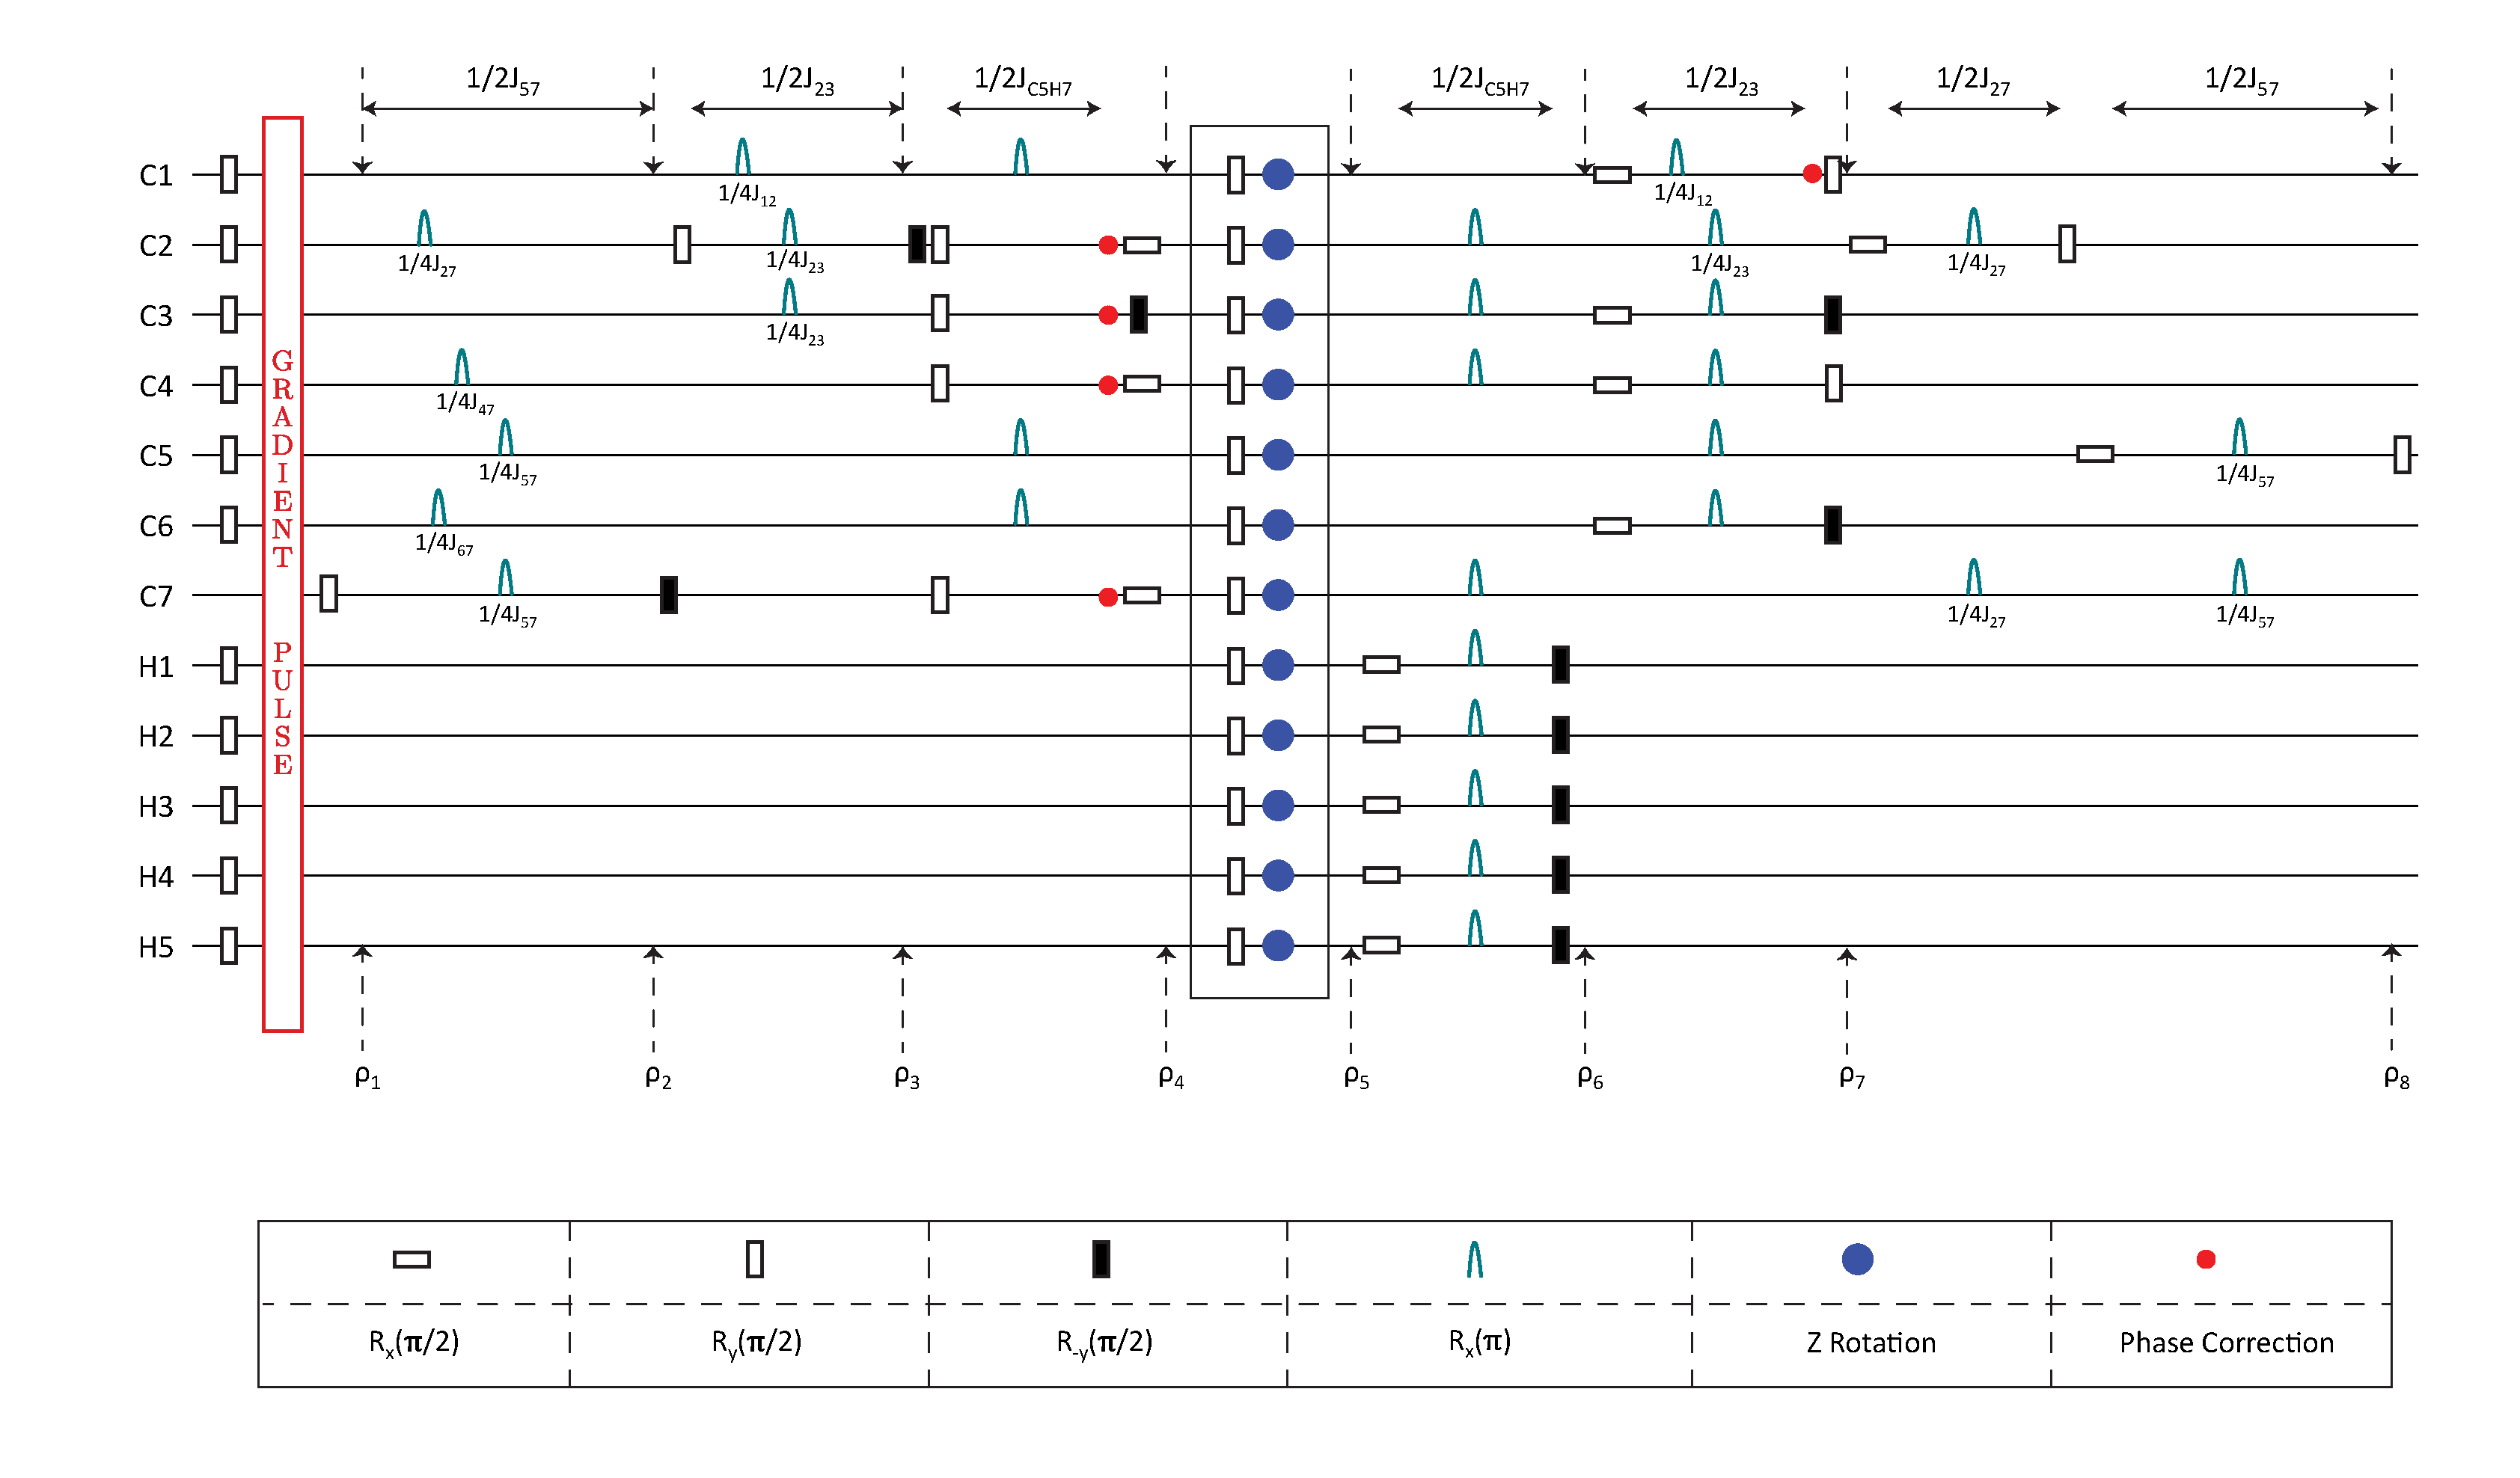
\includegraphics[width=\columnwidth]{12-spin-pps-circuit.pdf}
\end{center}
\setlength{\abovecaptionskip}{-0.35cm}
\caption{\footnotesize{Circuit to realize the 12-qubit PPS with some simplifications.}}\label{12-spin-pps-circuit}
\end{figure}

\begin{figure}[htb]
\begin{center}
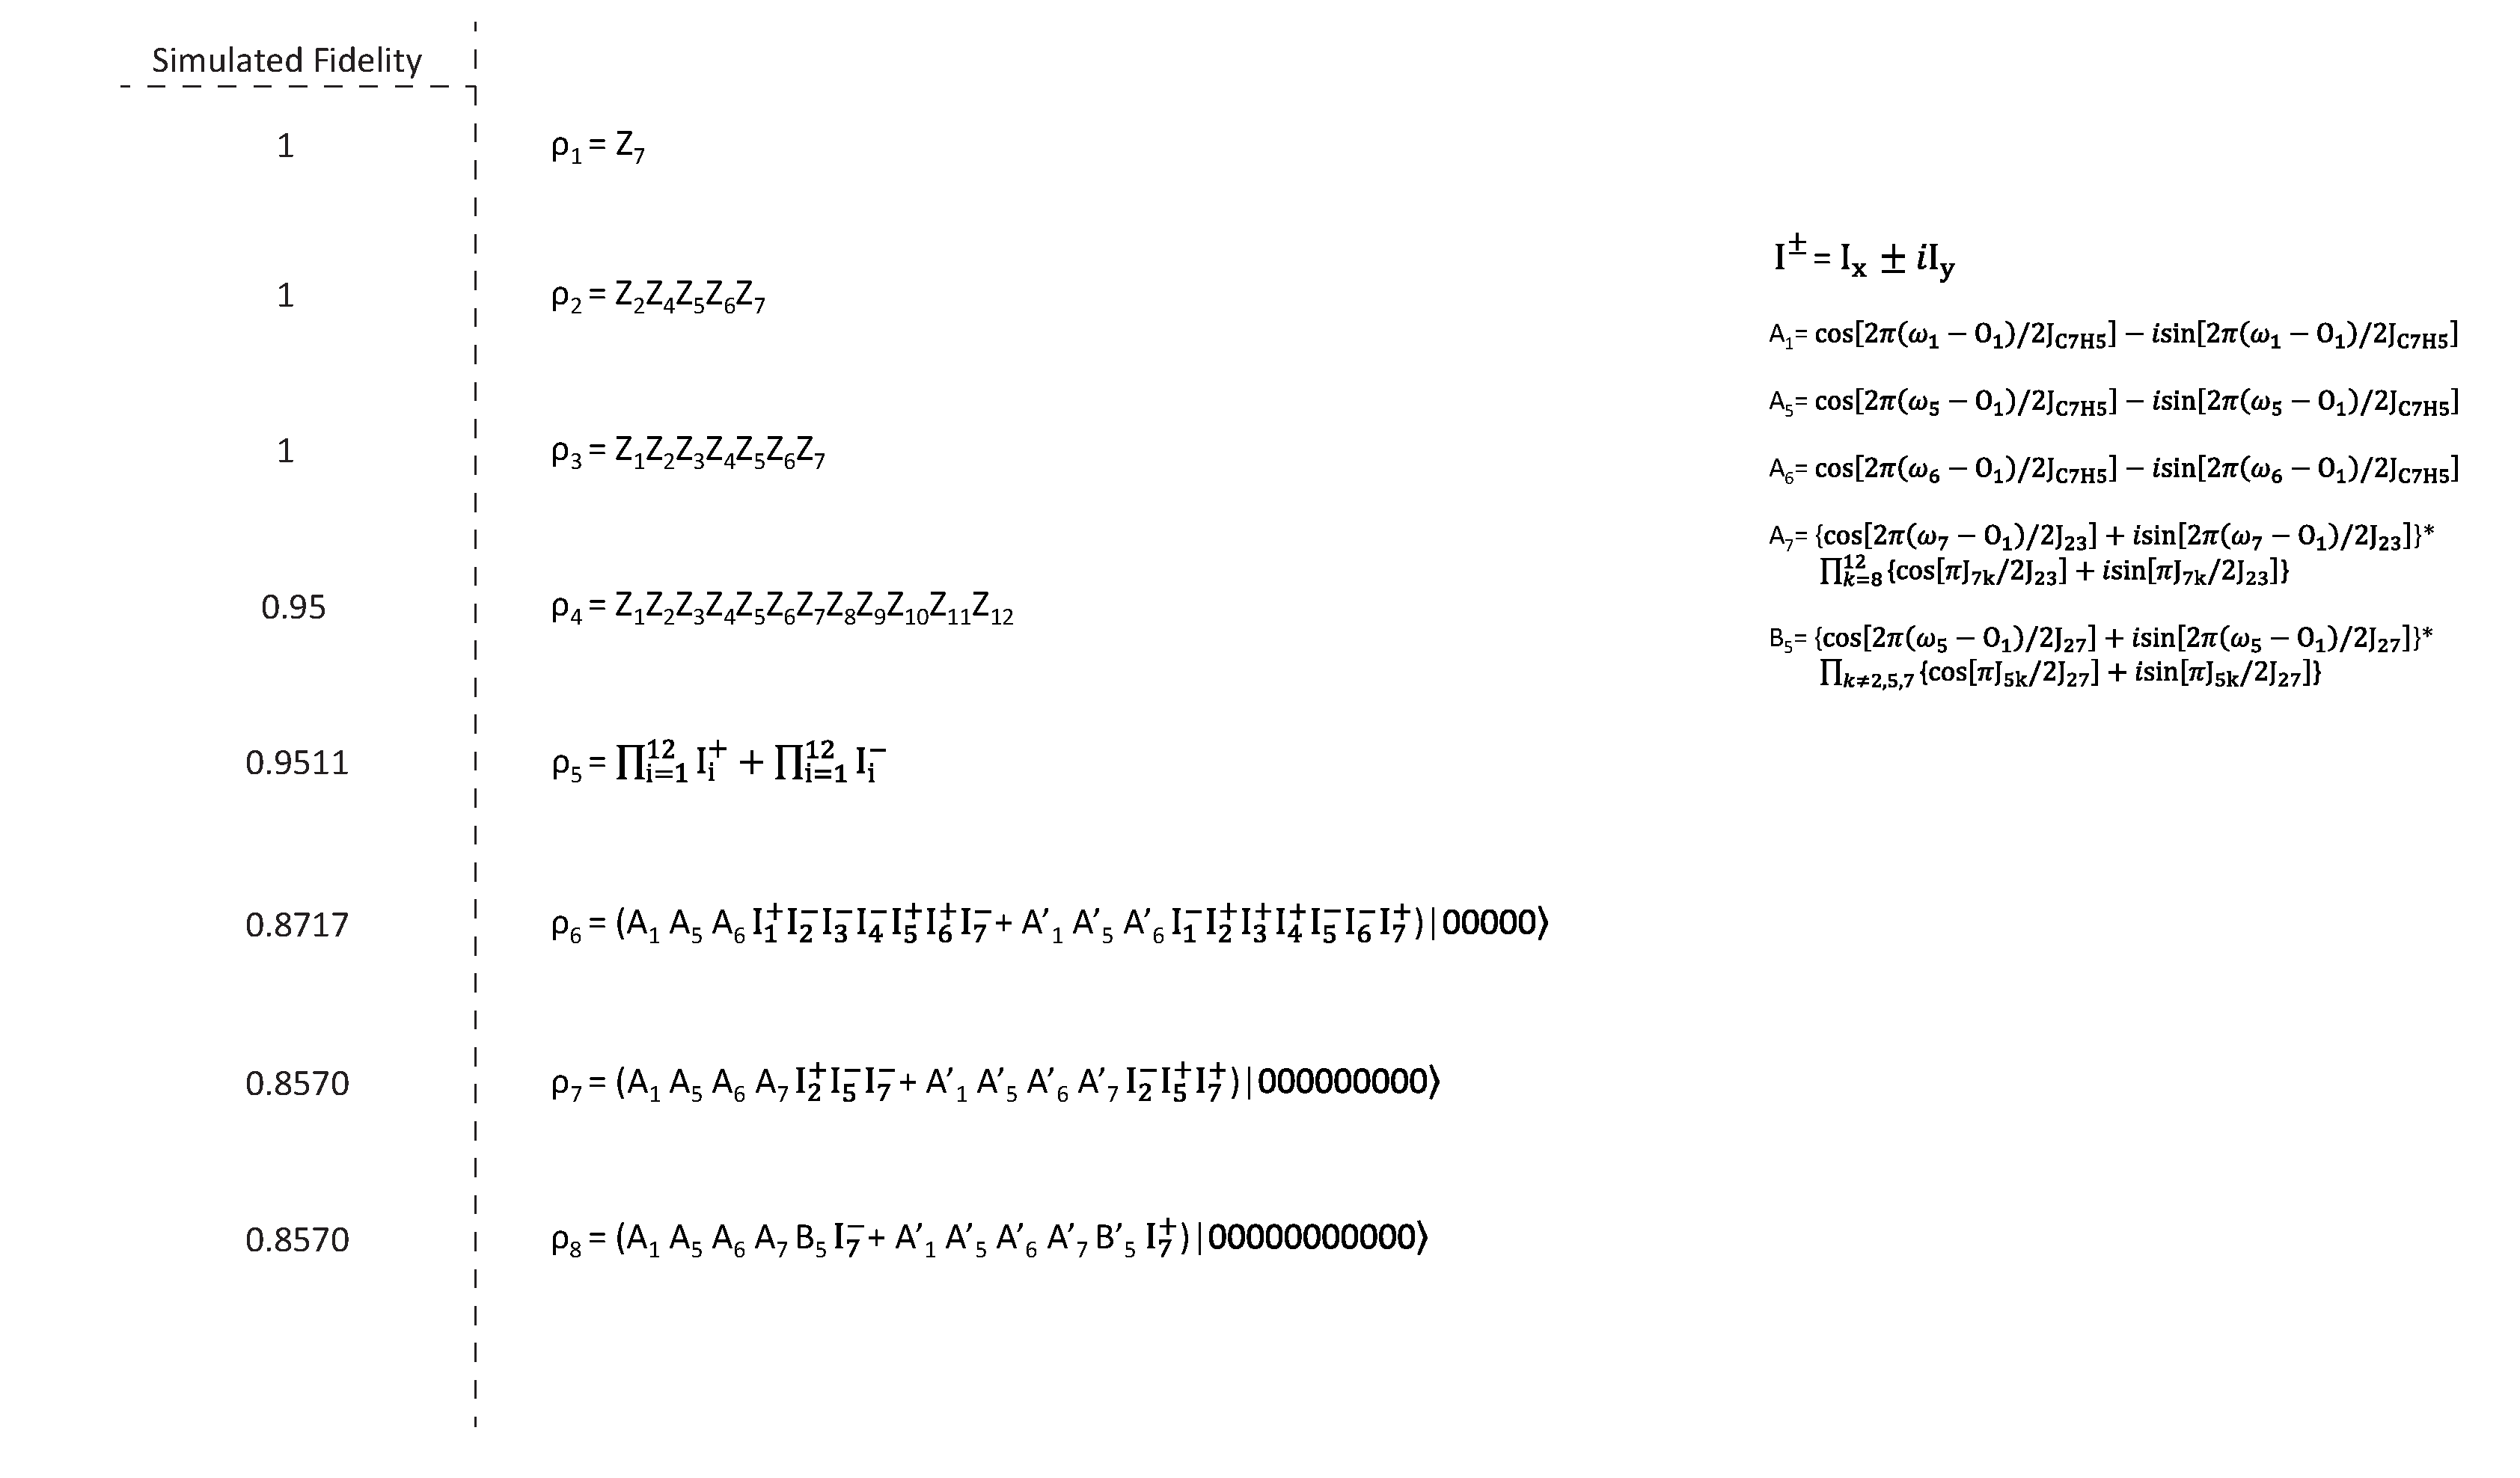
\includegraphics[width=\columnwidth]{circuit-simulation-result.pdf}
\end{center}
\setlength{\abovecaptionskip}{-0.35cm}
\caption{\footnotesize{States and fidelities after every step in the 12-qubit PPS circuit.}}\label{circuit-simulation-result}
\end{figure}

\clearpage
Exp 1401: Observe C7 by GRAPE as the reference. NS=10.\\
Exp 1402: Observe C2 by GRAPE as the reference. NS=10. \\

\begin{figure}[htb]
\begin{center}
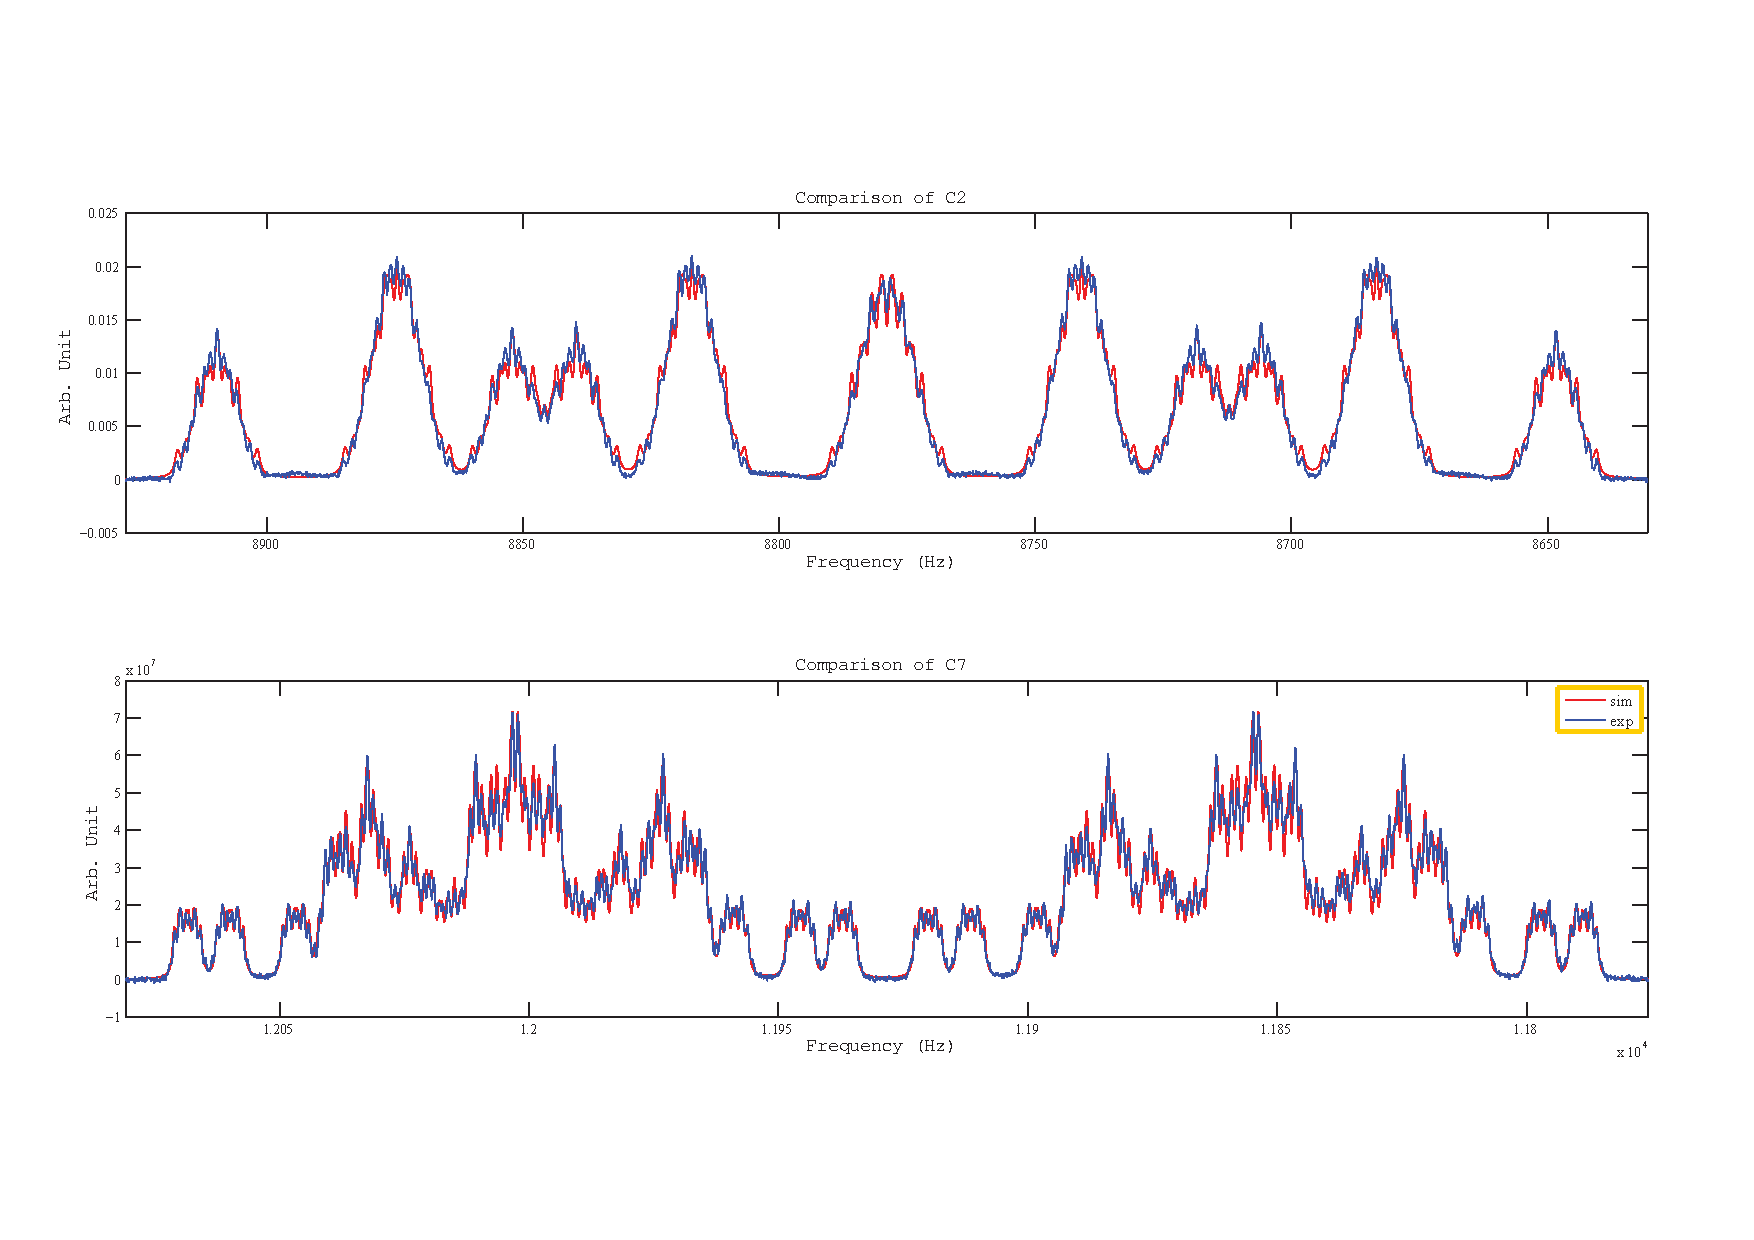
\includegraphics[width=\columnwidth]{Thermal_C2andC7.pdf}
\end{center}
\setlength{\abovecaptionskip}{-0.35cm}
\caption{\footnotesize{Comparison of the thermal for C2 and C7. Blue is experiment and Red is the simulation by the fitted Hamiltonian.}}\label{1401and1402}
\end{figure}

%\begin{figure}[htb]
%
%\centering
%\subfigure[Exp 1401 and 1402]{\label{1401and1402}
%\begin{minipage}[c]{\columnwidth}
%\centering
%  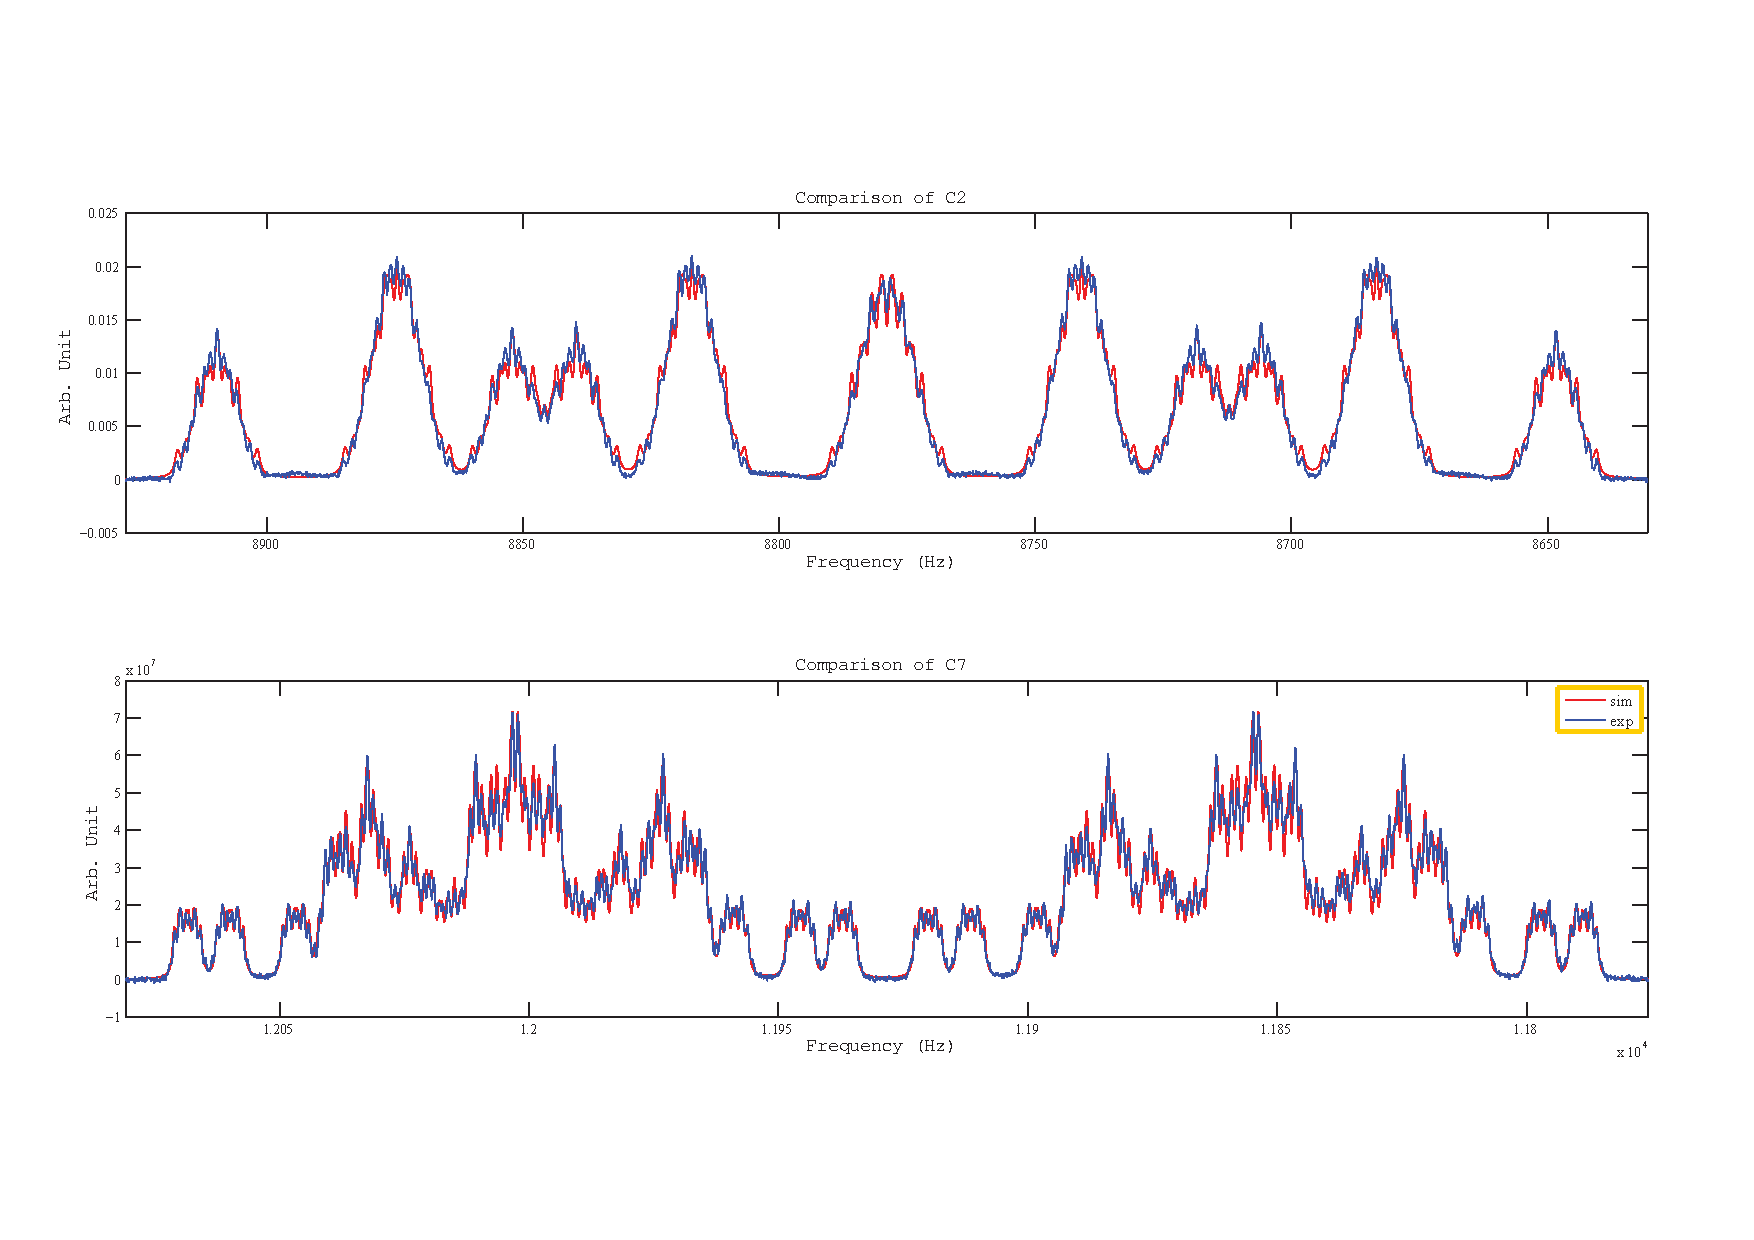
\includegraphics[width=0.8\columnwidth]{Thermal_C2andC7.pdf}
%\end{minipage}%
%}%
%
%\subfigure[Exp 2401 and 2402]{\label{2401and2402}
%\begin{minipage}[c]{\columnwidth}
%\centering
%  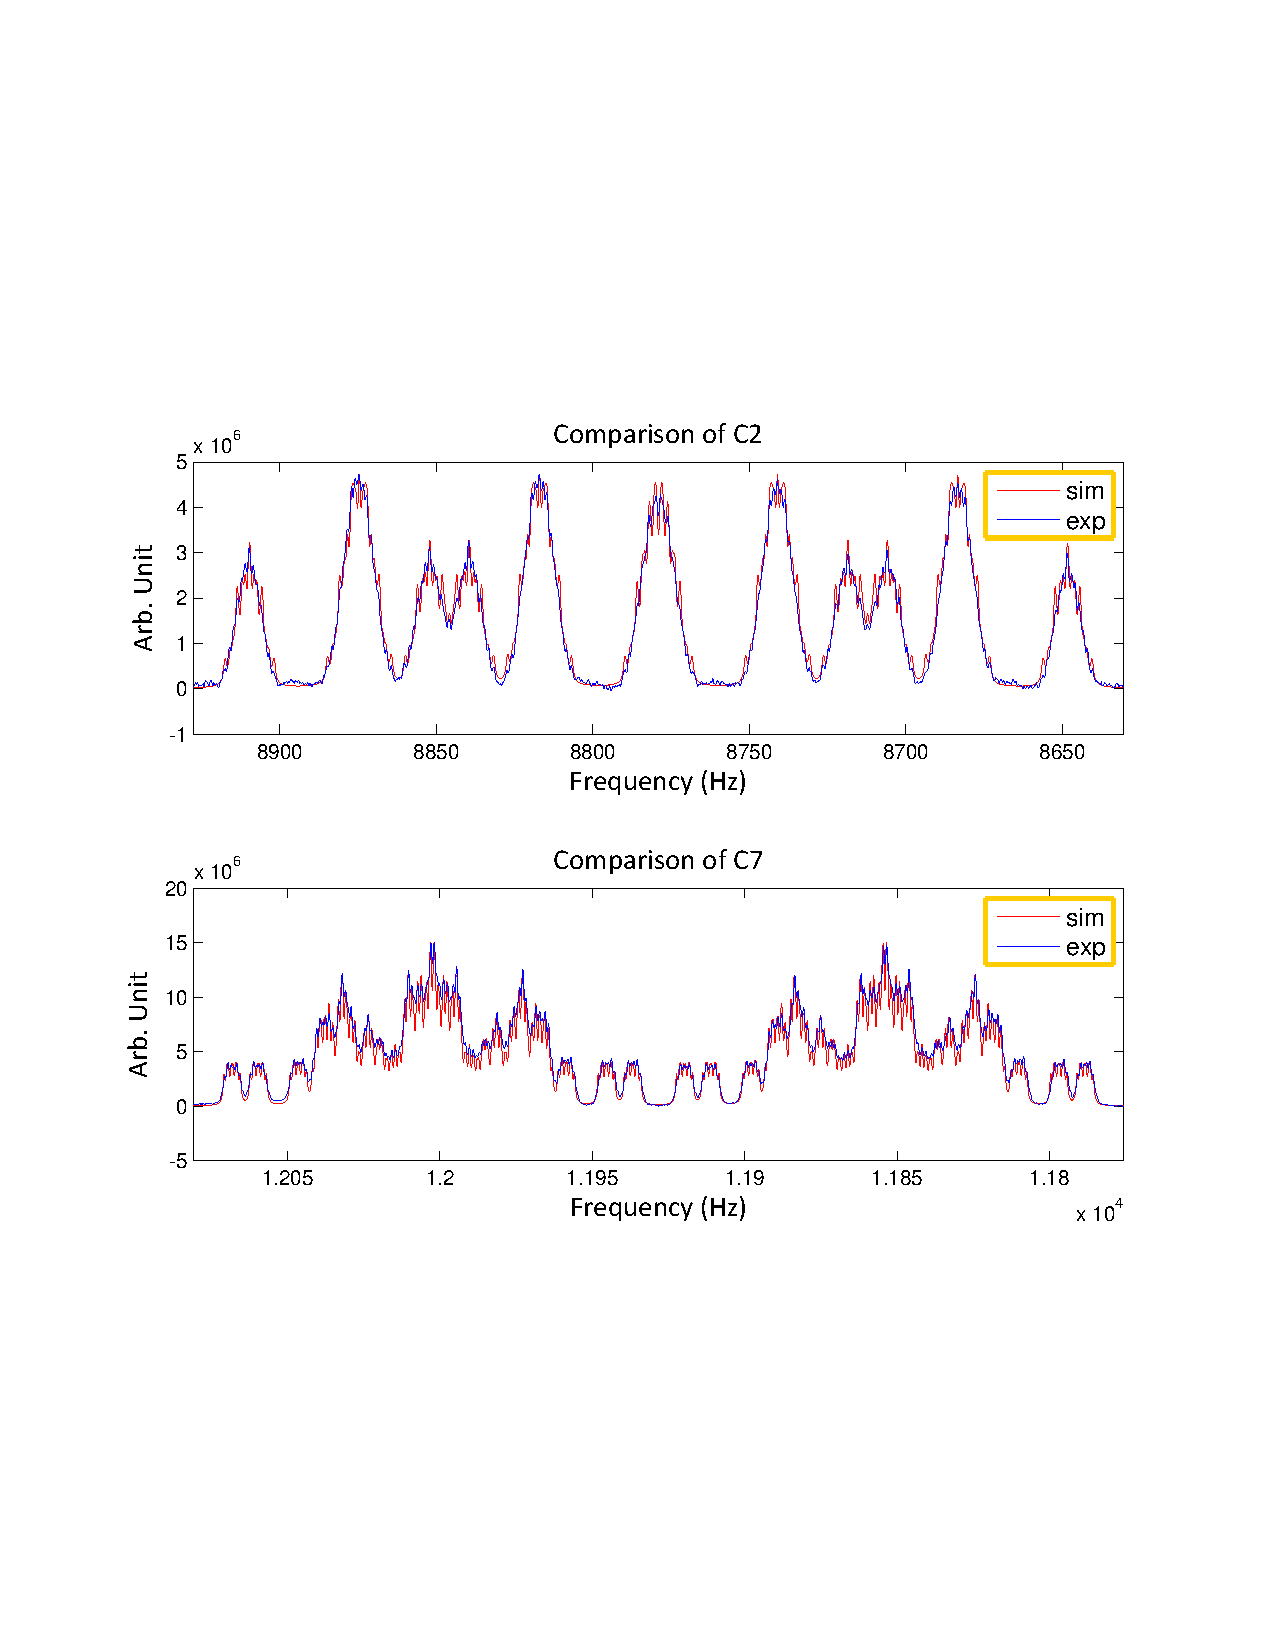
\includegraphics[width=0.8\columnwidth]{Thermal_C7SWAPandC2NoSWAP_Hcouple.pdf}
%\end{minipage}
%}
%\caption{\footnotesize{Comparison of the thermal for C2 and C7. Blue is experiment and Red is the simulation by the fitted Hamiltonian.}}\label{Thermal_C7SWAPandC2NoSWAP_Hcouple}
%\end{figure}

\clearpage
Exp 1403: Observe C7 after encoding1. NS=10.\\
Exp 1404: Observe C2 after encoding1. NS=10.\\

For C2 there is no signal because for Z24567 some couplings are close to 0 and the C2-H couplings broadens the peak. So for 12 qubits, these small couplings cannot be resolved.\\
For C7 it matches well with the simulation. However, the small couplings are annihilated due to the C7-H couplings too.

\begin{figure}[htb]
\begin{center}
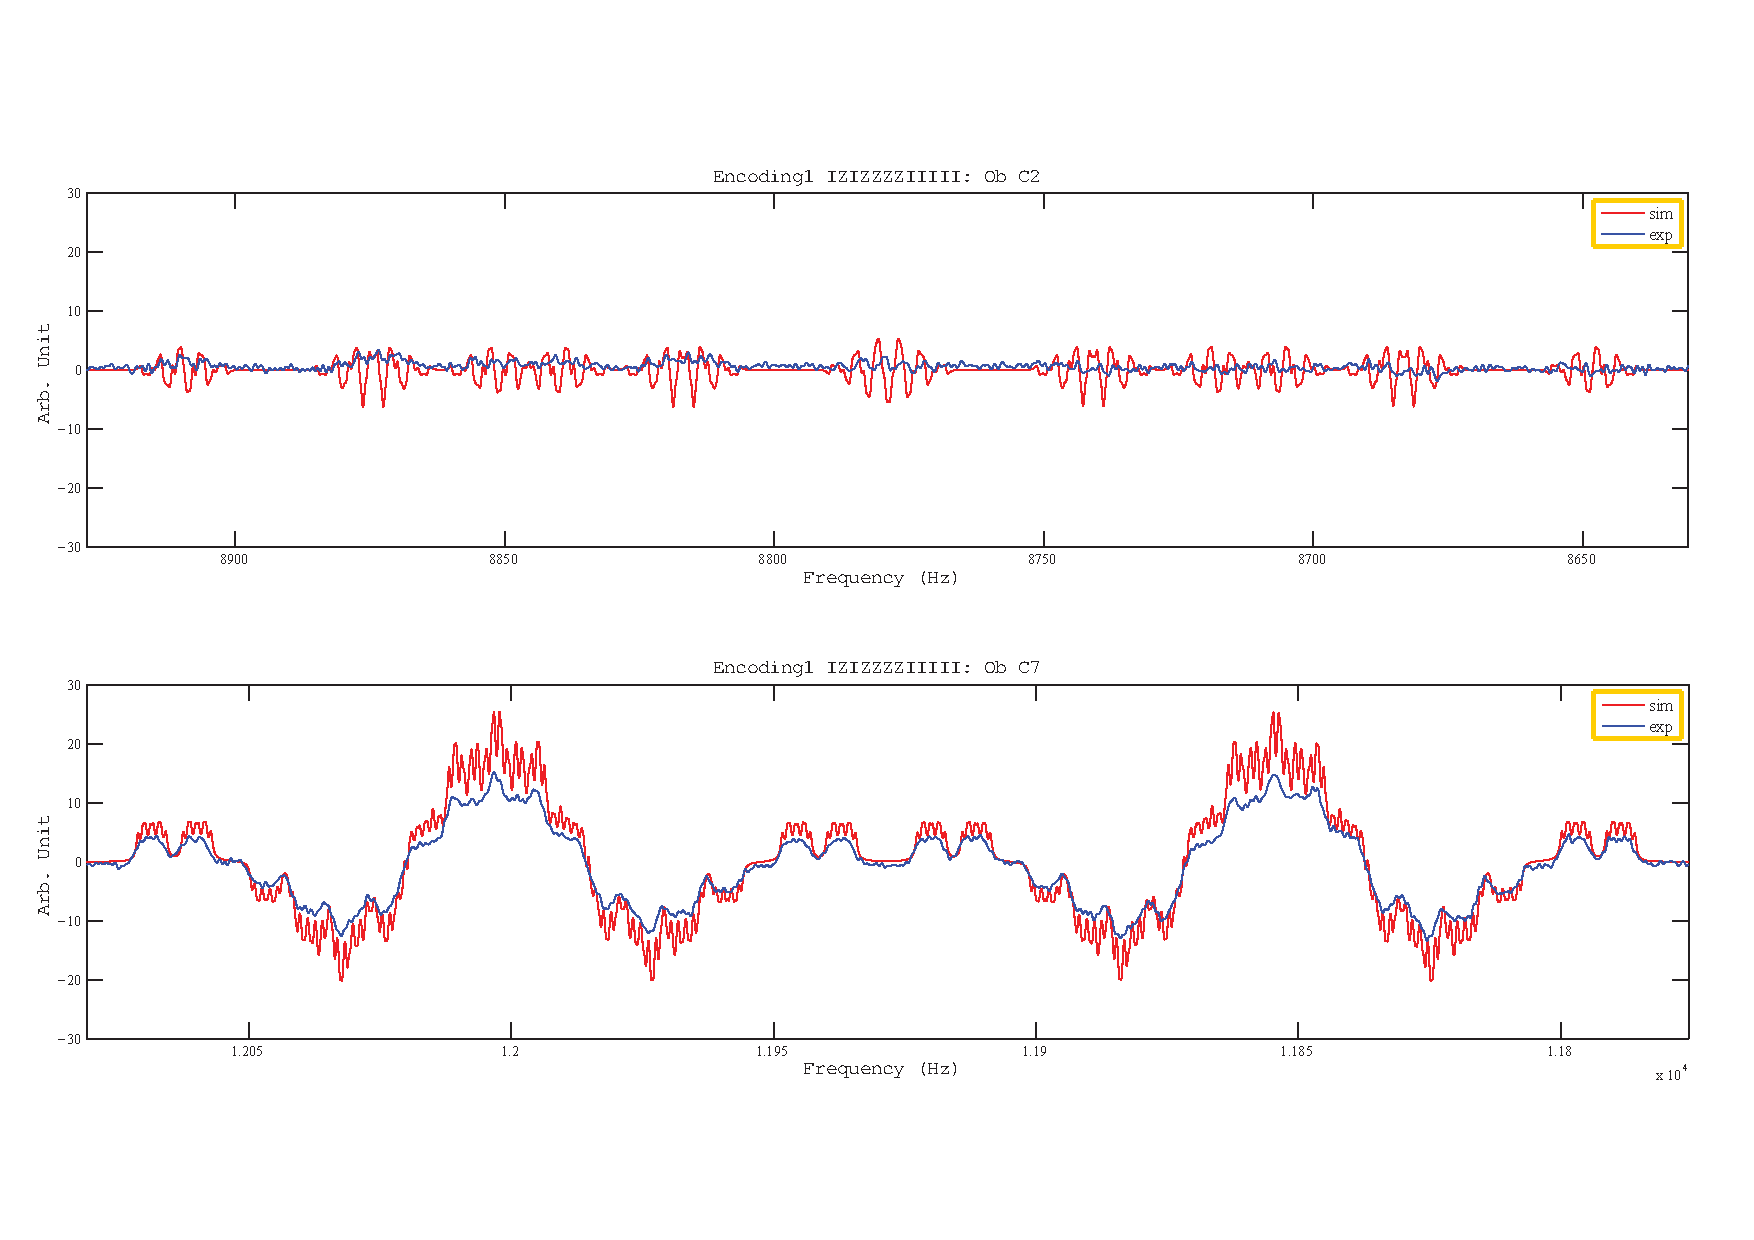
\includegraphics[width=\columnwidth]{Encoding1_without_decouple.pdf}
\end{center}
\setlength{\abovecaptionskip}{-0.35cm}
\caption{\footnotesize{Encoding 1 for C2 and C7 without H decoupled. 10 scans.}}\label{1403and1404}
\end{figure}

\clearpage
Exp 1405: Observe C7 after encoding1 and decouple H. NS=1.\\
Exp 1406: Observe C2 after encoding1 and decouple H. NS=1.\\
\textbf{Note compare with undecoupled experiments, for decoupling experiments I just used 1 scan.}

For C2 the signal is quite close to the 7-qubit case. Good.\\
For C7 the same.

\begin{figure}[htb]
\begin{center}
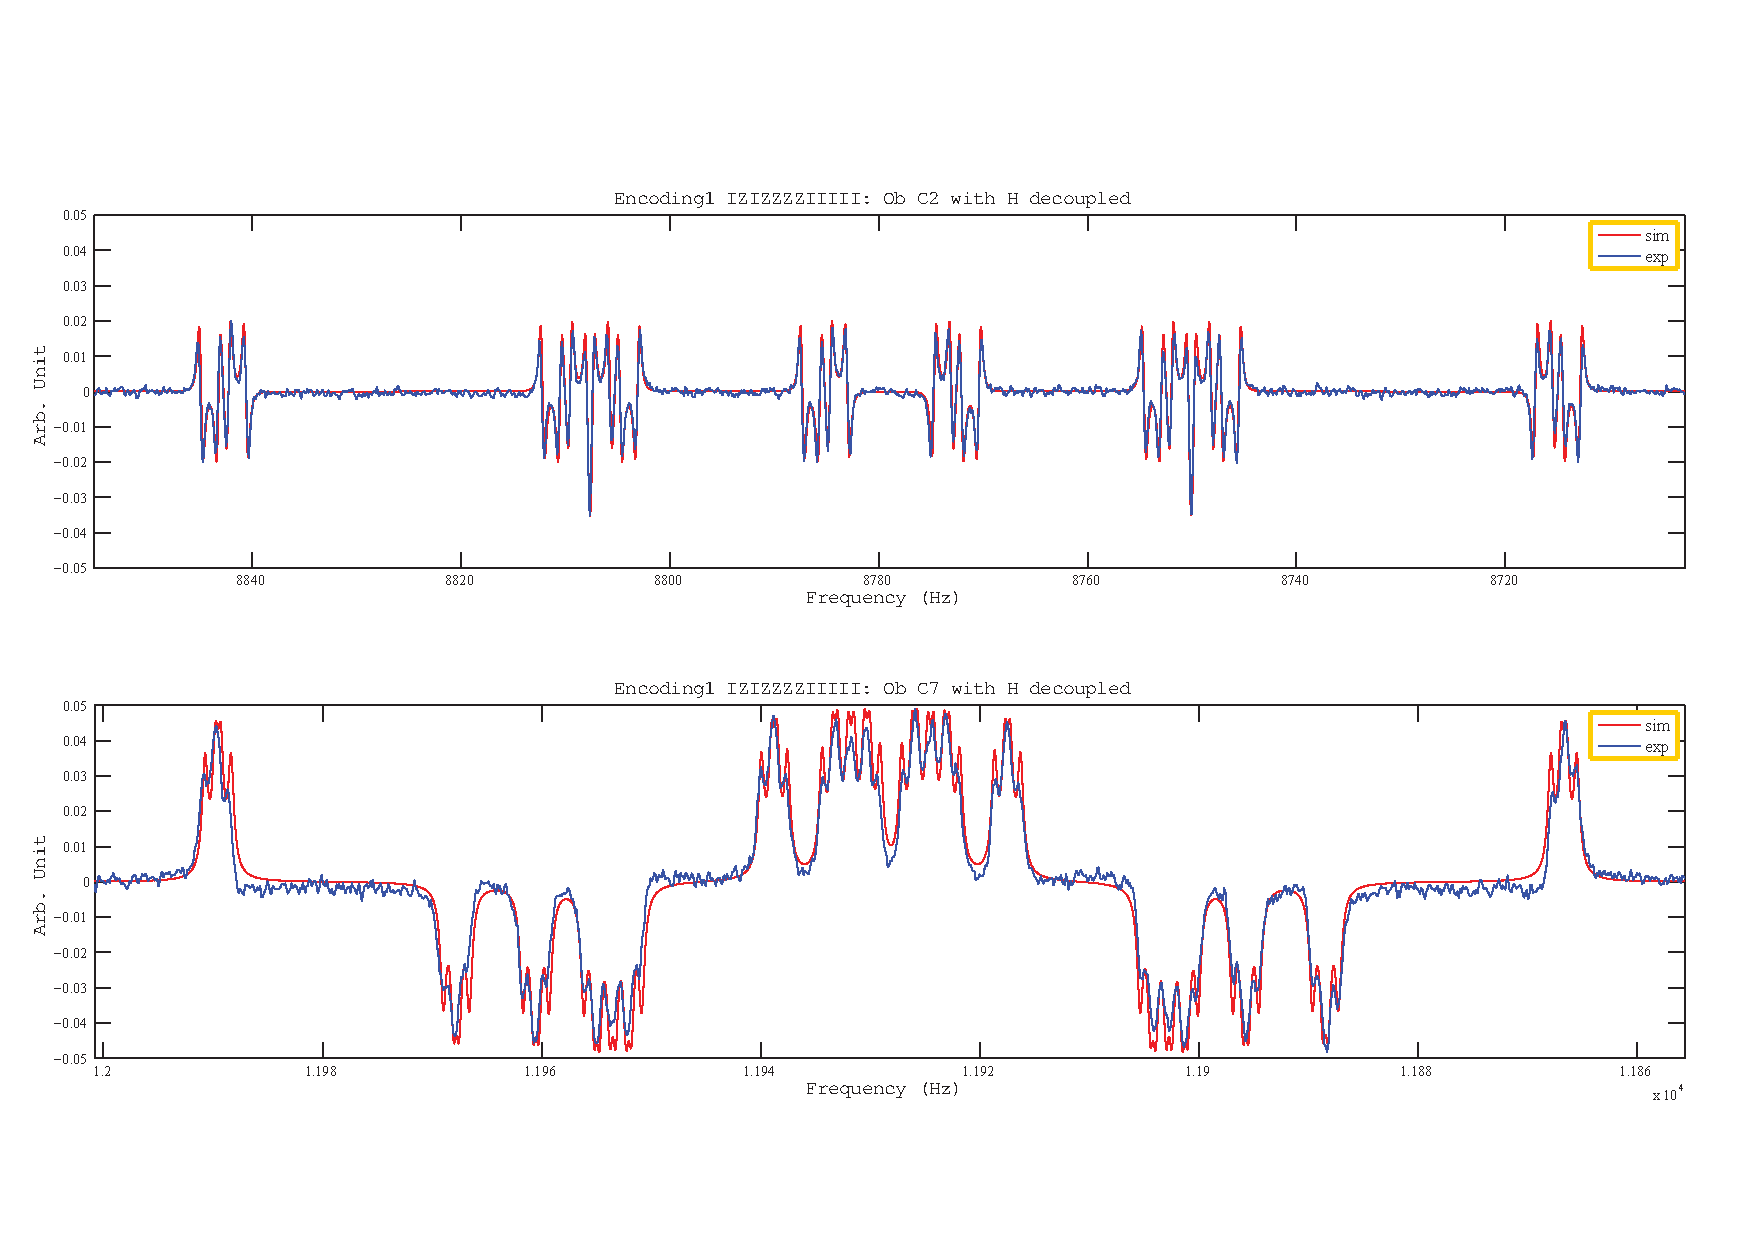
\includegraphics[width=\columnwidth]{Encoding1_with_decouple.pdf}
\end{center}
\setlength{\abovecaptionskip}{-0.35cm}
\caption{\footnotesize{Encoding 1 for C2 and C7 with H decoupled. 1 scan.}}\label{1405and1406}
\end{figure}

\clearpage
Exp 1407: Observe C7 after encoding2. NS=10.\\
Exp 1408: Observe C2 after encoding2. NS=10.\\

For C2 and C7 there are no signals due to the broaden of the C-H couplings.

\begin{figure}[htb]
\begin{center}
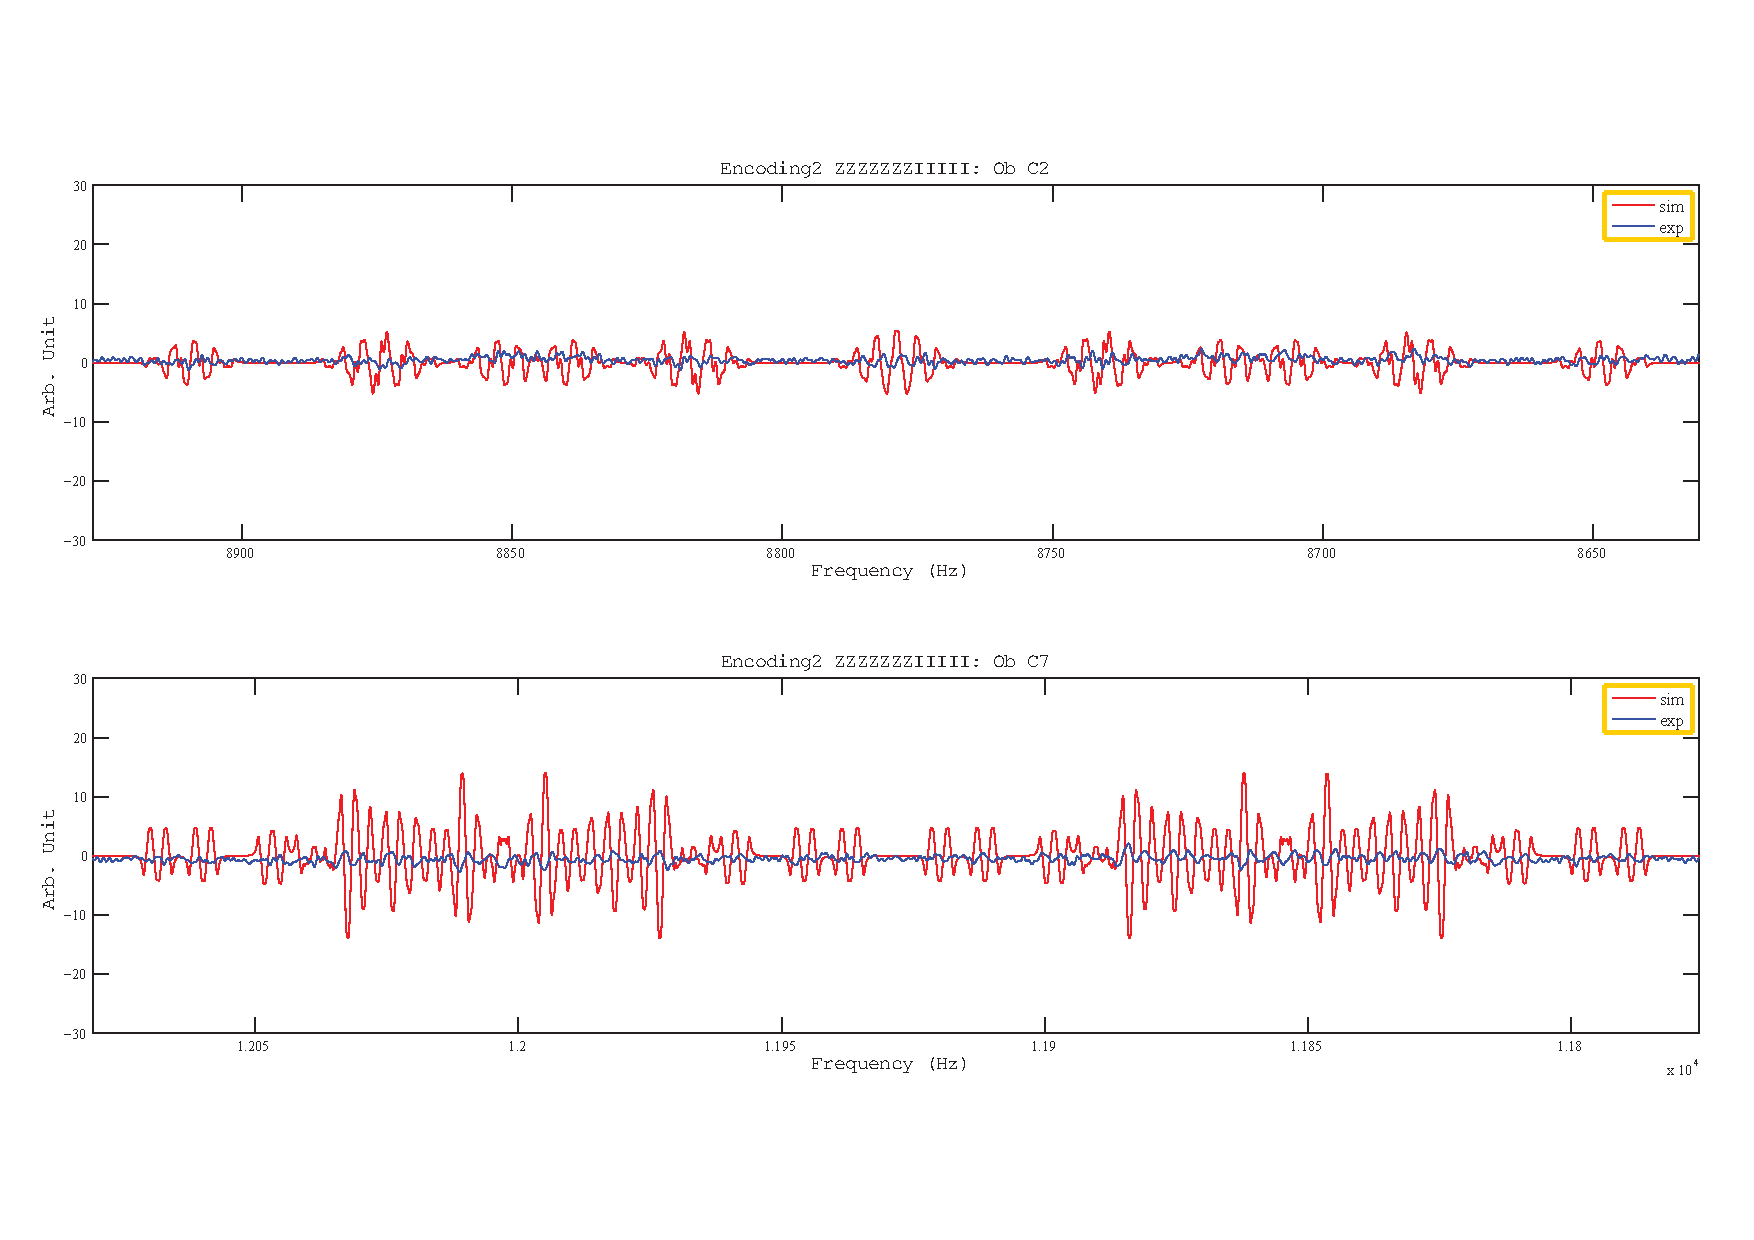
\includegraphics[width=\columnwidth]{Encoding2_without_decouple.pdf}
\end{center}
\setlength{\abovecaptionskip}{-0.35cm}
\caption{\footnotesize{Encoding 2 for C2 and C7 without H decoupled. 10 scans.}}\label{1407and1408}
\end{figure}

\clearpage
Exp 1409: Observe C7 after encoding2 and decouple H. NS=1.\\
Exp 1410: Observe C2 after encoding2 and decouple H. NS=1.\\
\textbf{Note compare with undecoupled experiments, for decoupling experiments I just used 1 scan.}

For C2 and C7 they both look nice.

\begin{figure}[htb]
\begin{center}
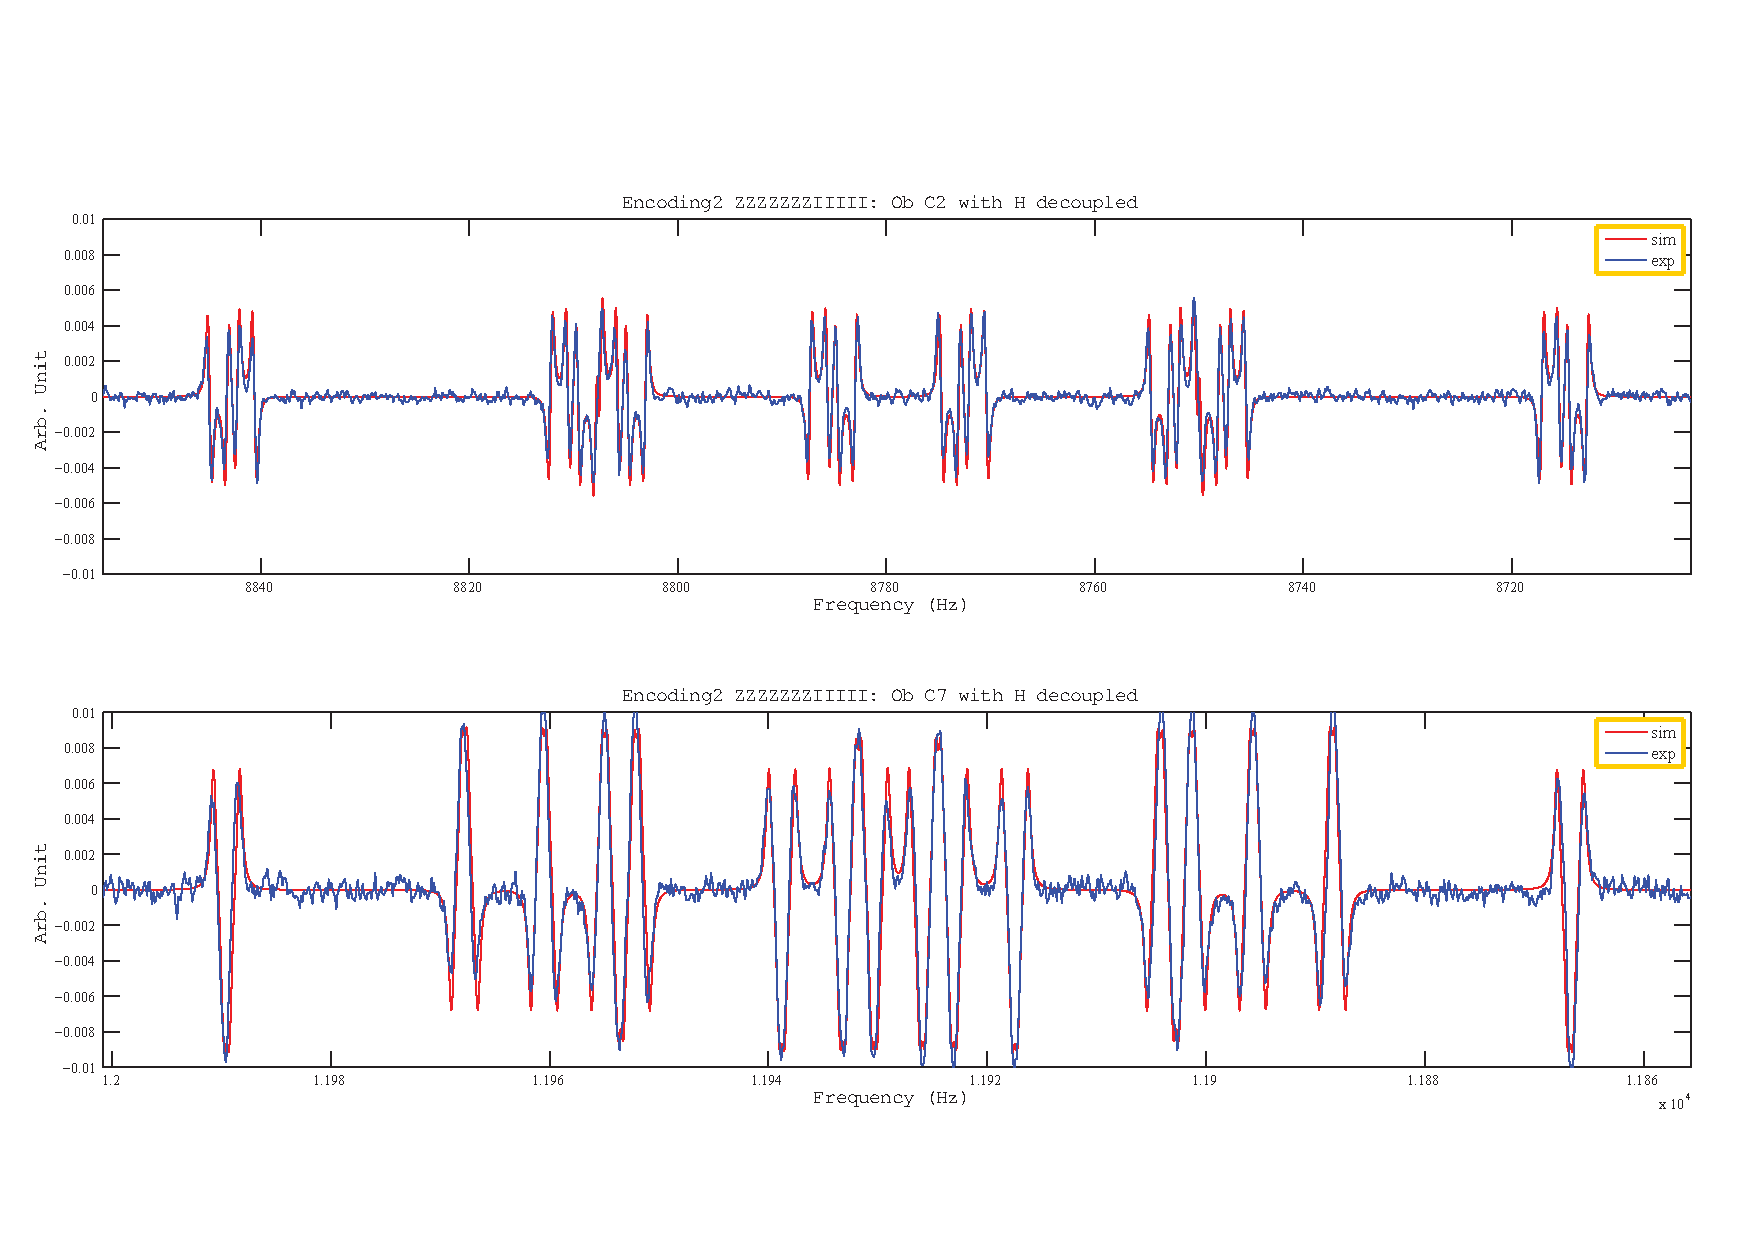
\includegraphics[width=\columnwidth]{Encoding2_with_decouple.pdf}
\end{center}
\setlength{\abovecaptionskip}{-0.35cm}
\caption{\footnotesize{Encoding 2 for C2 and C7 with H decoupled. 1 scan.}}\label{1409and1410}
\end{figure}

\clearpage
Exp 1411: Observe C7 after encoding3. Encoding 3 is applied on thermal. NS=1.\\
Exp 1412: Observe C2 after encoding3. Encoding 3 is applied on thermal. NS=1.\\
\textbf{Note the encoding 3 operator is just applied on thermal because if it is applied consequently after encoding 2 the spectra has no signal.}

They look okay as I did not adjust the experimental parameters much. In principal, only C-H will be anti-phase.

\begin{figure}[htb]
\begin{center}
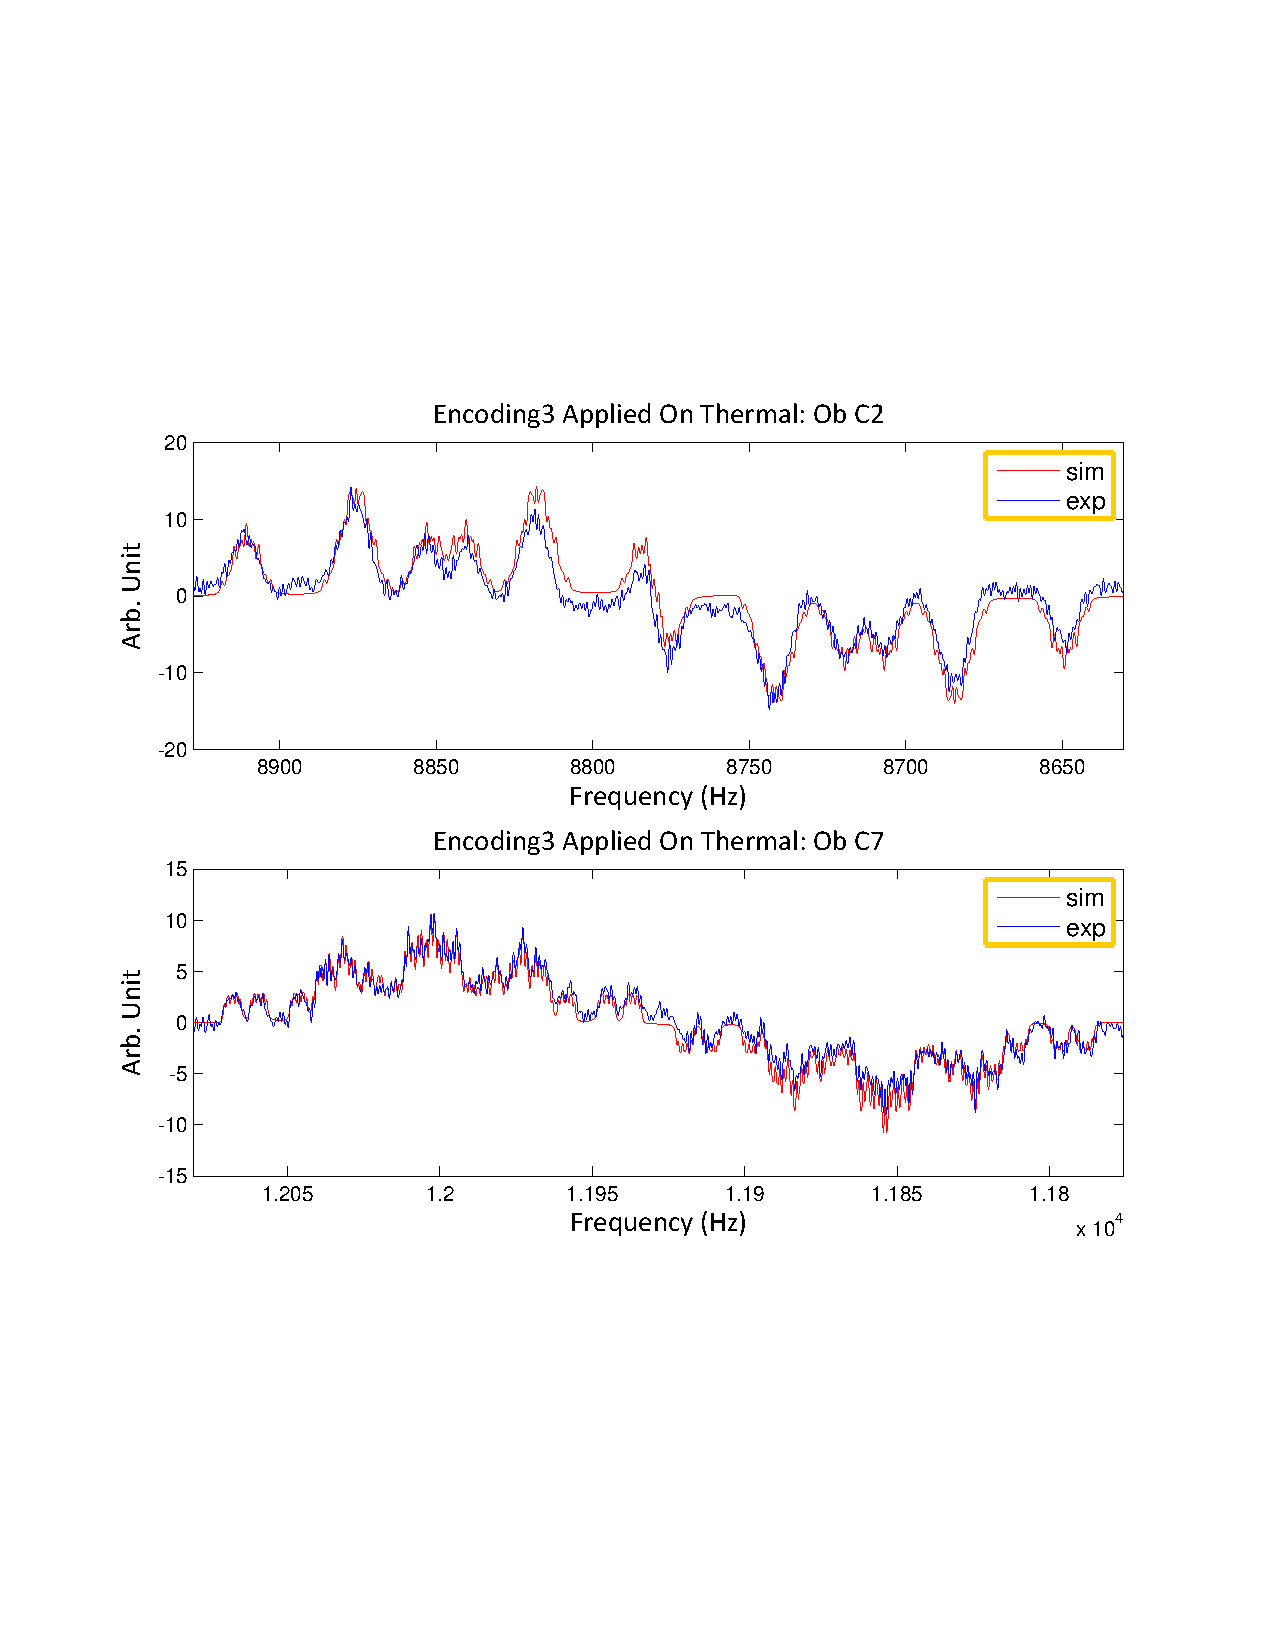
\includegraphics[width=\columnwidth]{Encoding3_without_decouple.pdf}
\end{center}
\setlength{\abovecaptionskip}{-0.35cm}
\caption{\footnotesize{Encoding 3 for C2 and C7 applied on thermal. 1 scan.}}\label{1411and1412}
\end{figure}

\clearpage
Exp 1887: Observe C7 on thermal. NS=7.\\
Exp 1888: Observe C7 after C-H SWAP applied on thermal. NS=7.\\

\begin{figure}[htb]
\begin{center}
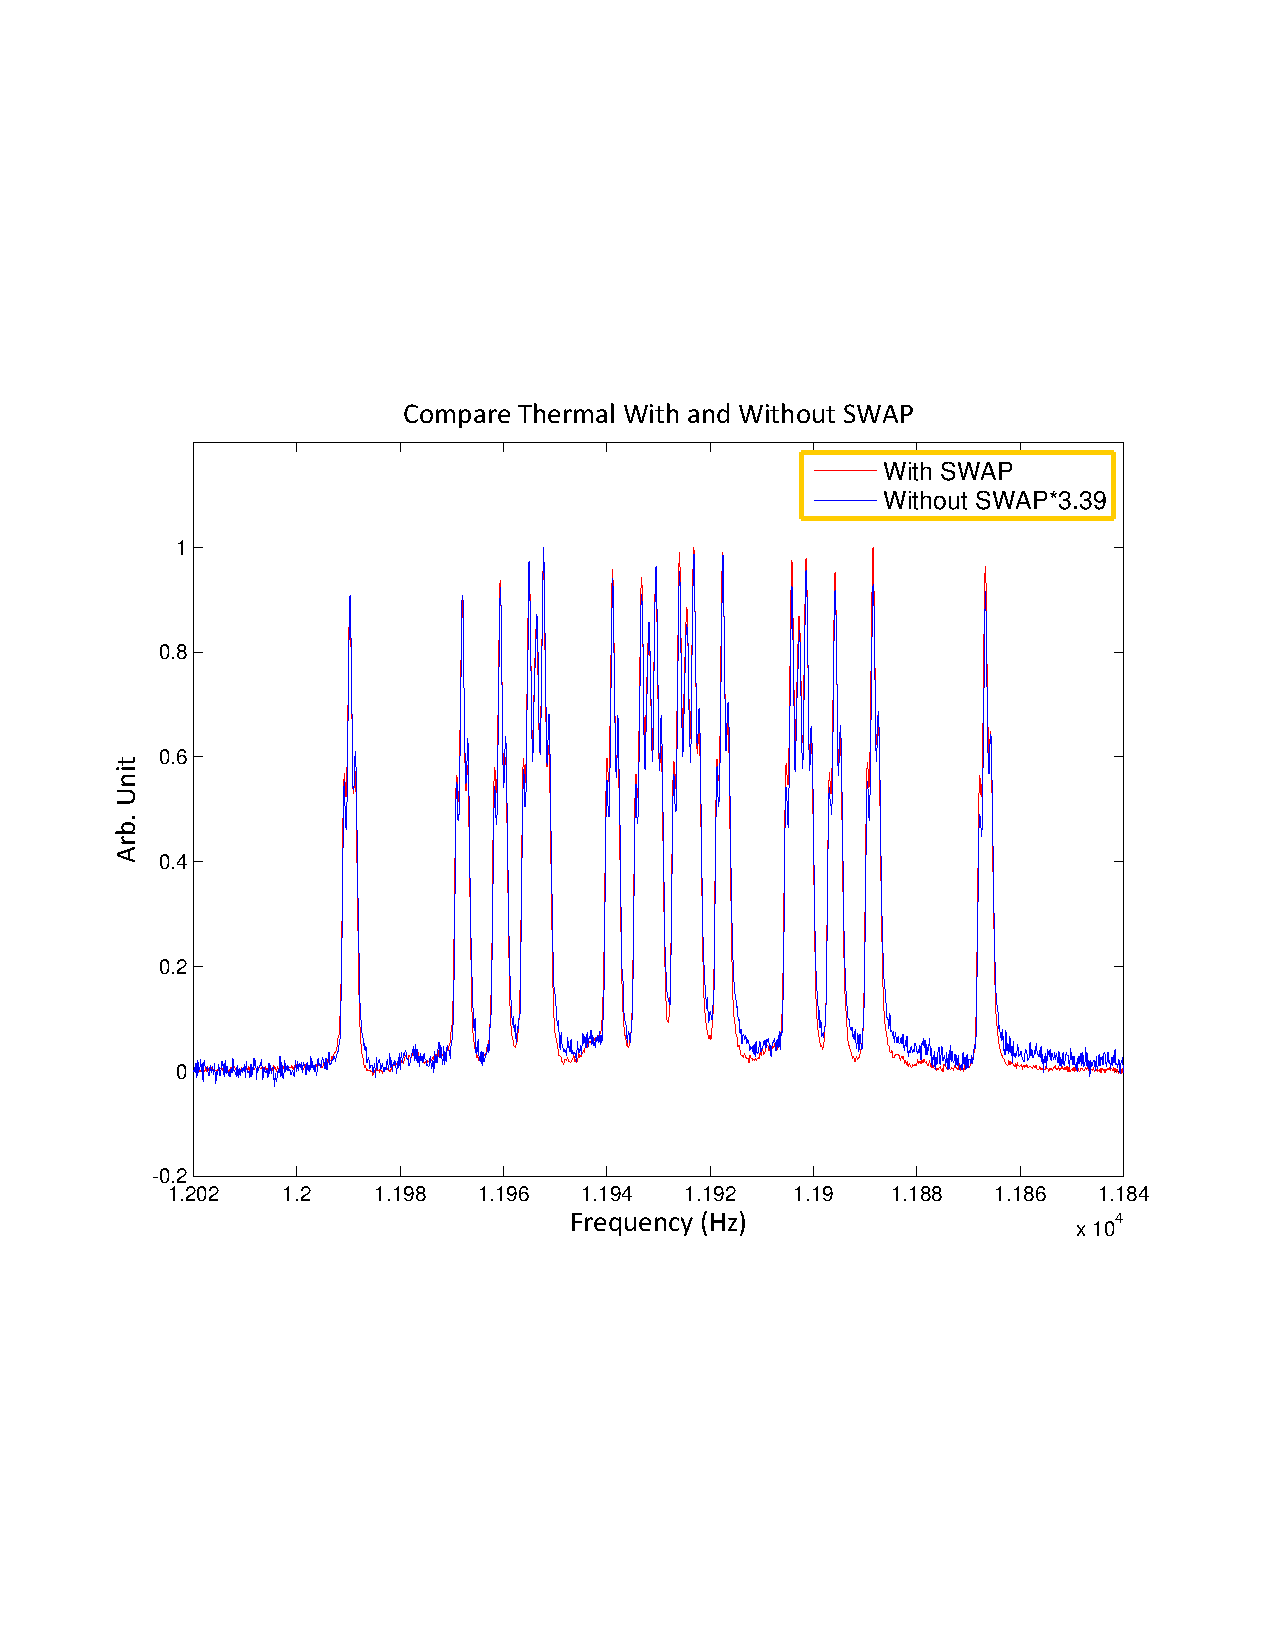
\includegraphics[width=\columnwidth]{Compare_Thermal_with_and_without_SWAP.pdf}
\end{center}
\setlength{\abovecaptionskip}{-0.35cm}
\caption{\footnotesize{Thermal spectrum with and without the C-H SWAP gate. The one with SWAP is 3.39 times higher.}}\label{1887and1888}
\end{figure}

\clearpage
Exp 1888: Observe C7 after C-H SWAP applied on thermal. NS=7.\\
Exp 1889: Observe C7 of the 7-qubit PPS. NS=7.\\

\begin{figure}[htb]
\begin{center}
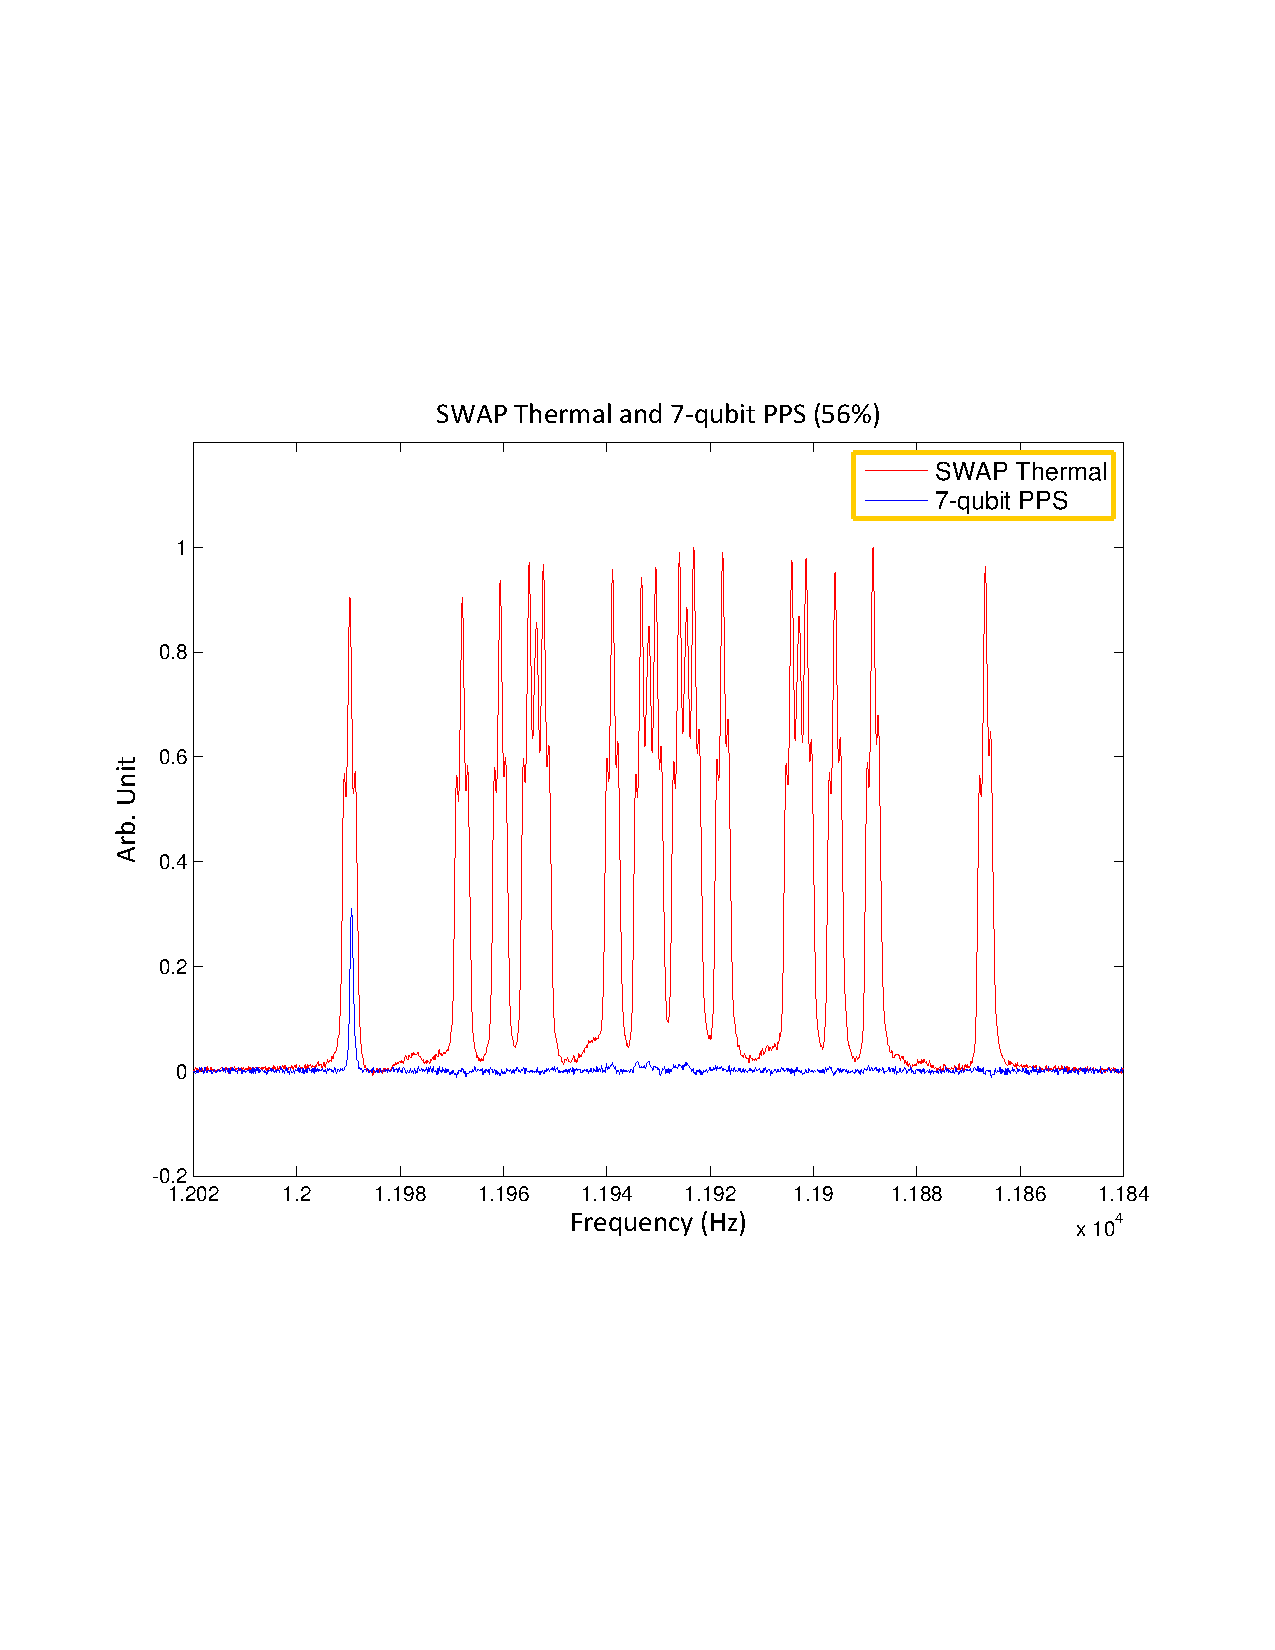
\includegraphics[width=\columnwidth]{SWAP_Thermal_and_7-qubit_PPS.pdf}
\end{center}
\setlength{\abovecaptionskip}{-0.35cm}
\caption{\footnotesize{Comparison between the thermal after C-H SWAP gate and the 7-qubit PPS. The remained signal of the PPS in contrast to the theory is 56\%.}}\label{1888and1889}
\end{figure}

\clearpage
Exp 1889: Observe C7 of the 7-qubit PPS. NS=7.\\
Exp 1891: Observe C7 of the 7-qubit PPS, with the Encoding replaced by 12-qubit pulses. NS=7.\\
Exp 1893: Observe C7 of the 7-qubit PPS, with the Encoding and Phase Cycling replaced by 12-qubit pulses. NS=7.\\

\begin{figure}[htb]
\begin{center}
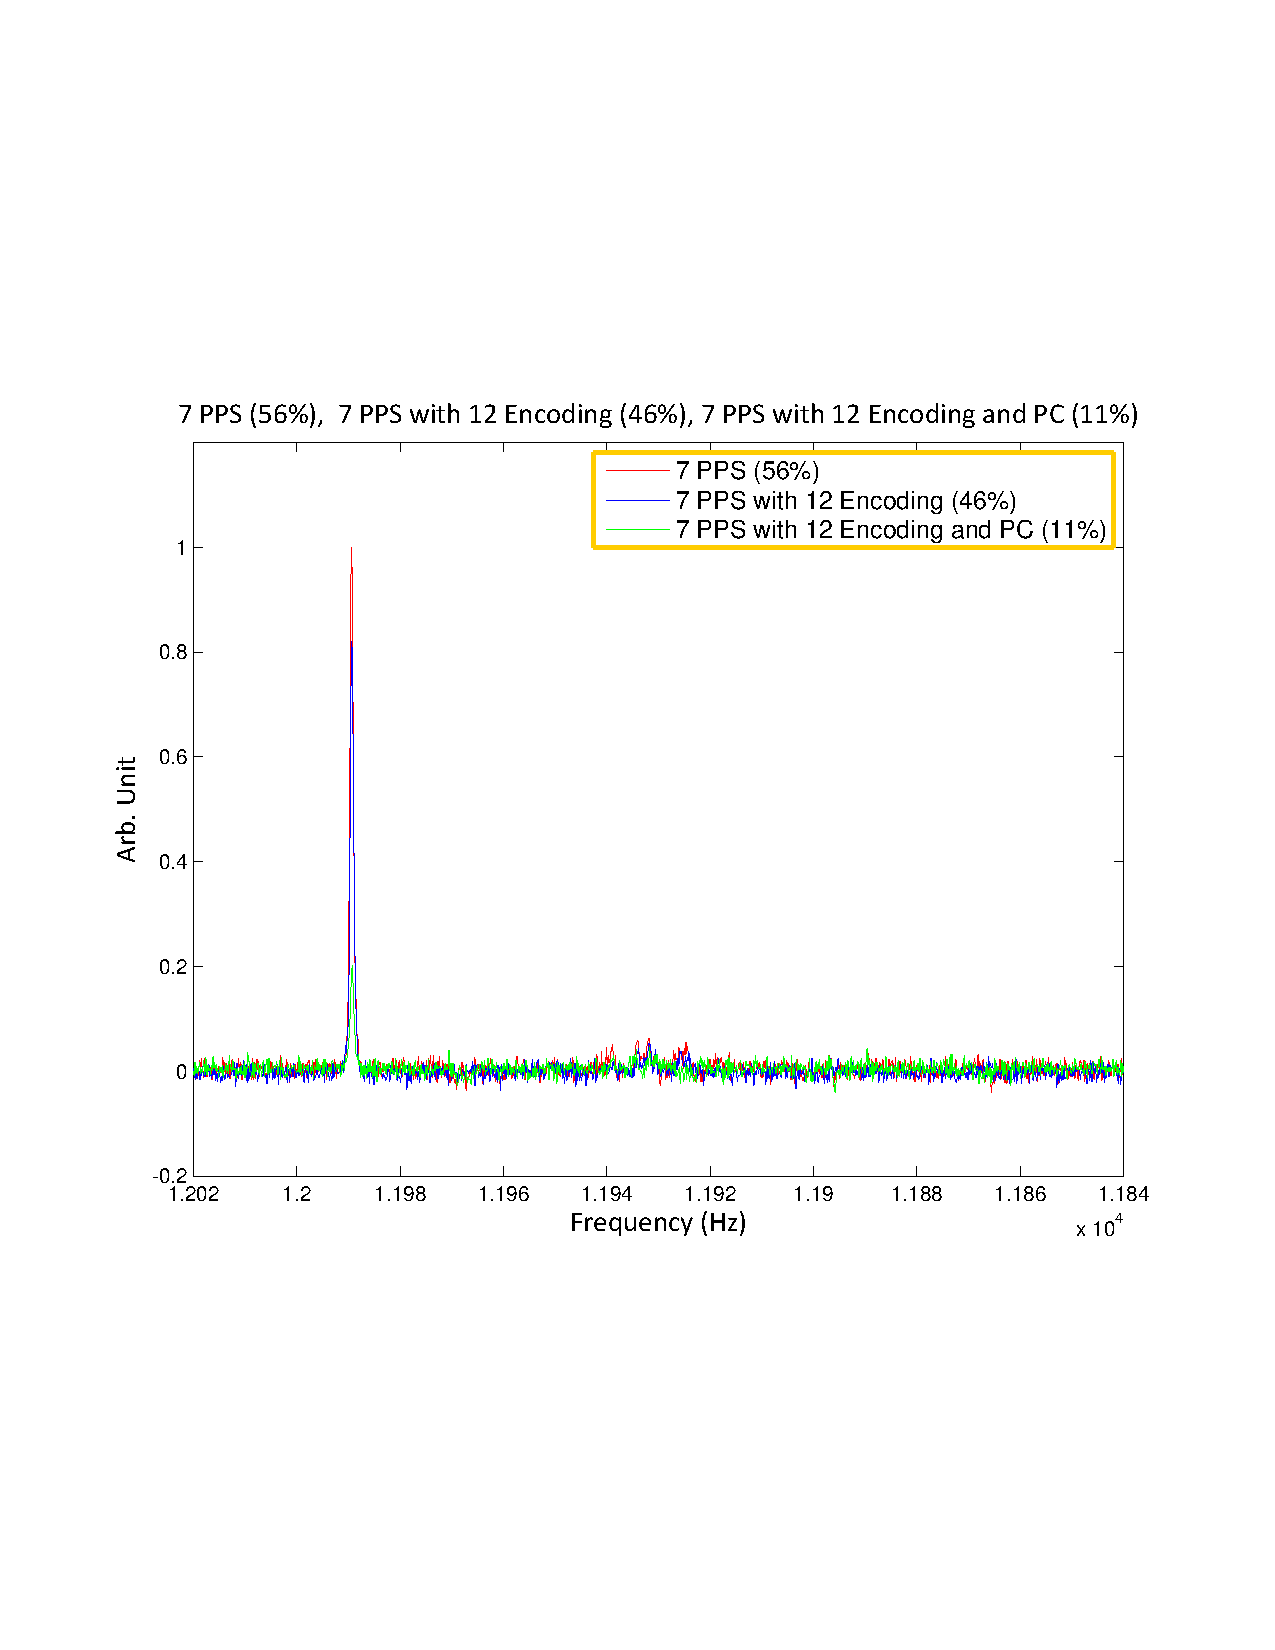
\includegraphics[width=\columnwidth]{7PPS_7PPSwith12Encoding_7PPSwith12EncodingandPC.pdf}
\end{center}
\setlength{\abovecaptionskip}{-0.35cm}
\caption{\footnotesize{Red: the original 7-qubit PPS (56\% compared to thermal); Blue: the 7-qubit PPS with the 12-qubit Encoding pulses (46\% compared to thermal). Green: the 7-qubit PPS with the 12-qubit Encoding and Phase Cycling pulses (11\% compared to thermal)}}\label{1889and1891and1893}
\end{figure} 

\clearpage
Exp 2401: Observe C7 by GRAPE as the reference. NS=10.\\
Exp 2402: Observe C2 by GRAPE as the reference. NS=10. \\

Exp 2401 is obtained after C-H SWAP gate.\\
Exp 2402 has no SWAP gate in the beginning.\\

\begin{figure}[htb]
\begin{center}
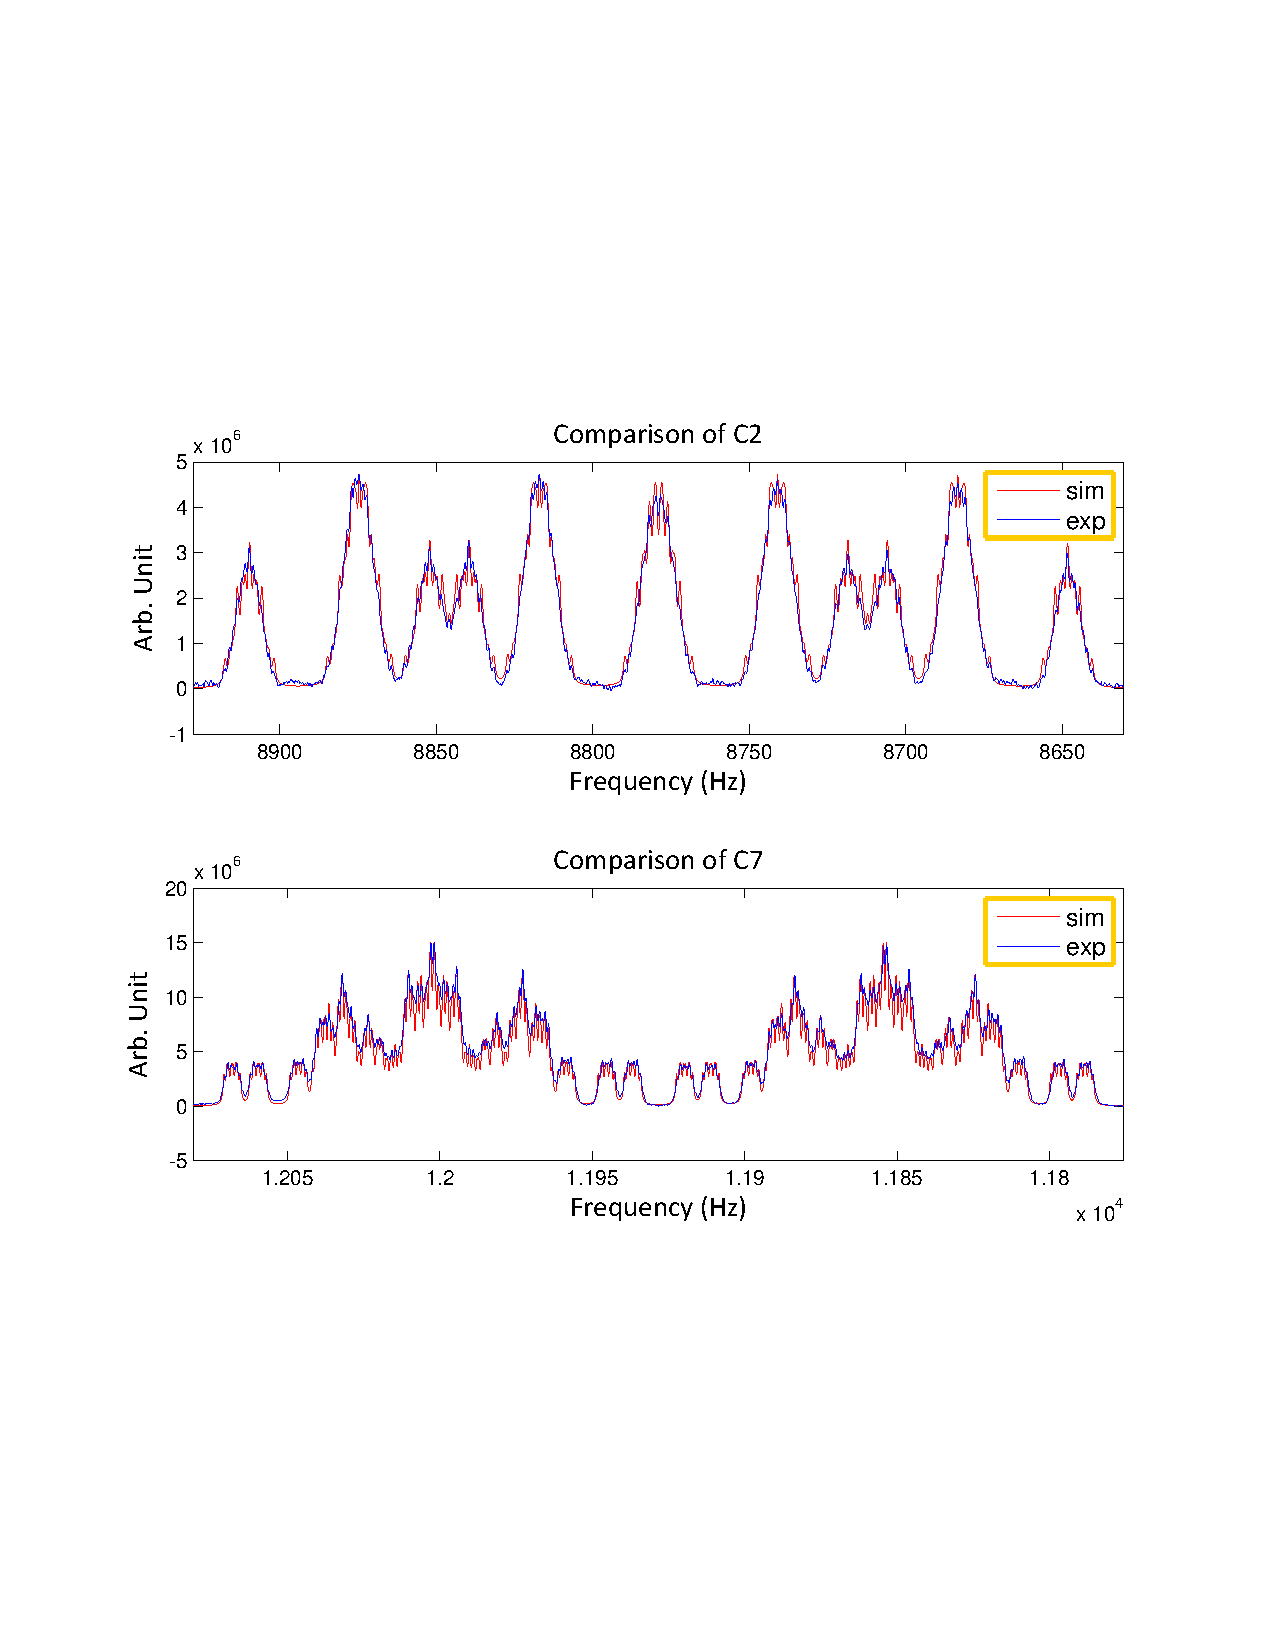
\includegraphics[width=\columnwidth]{Thermal_C7SWAPandC2NoSWAP_Hcouple.pdf}
\end{center}
\setlength{\abovecaptionskip}{-0.35cm}
\caption{\footnotesize{Comparison of the thermal for C2 and C7. Blue is experiment and Red is the simulation by the fitted Hamiltonian.}}\label{2401and2402}
\end{figure}

\clearpage
Exp 2403: Observe C7 after encoding1. NS=10.\\
Exp 2404: Observe C2 after encoding1. NS=10.\\

\begin{figure}[htb]
\begin{center}
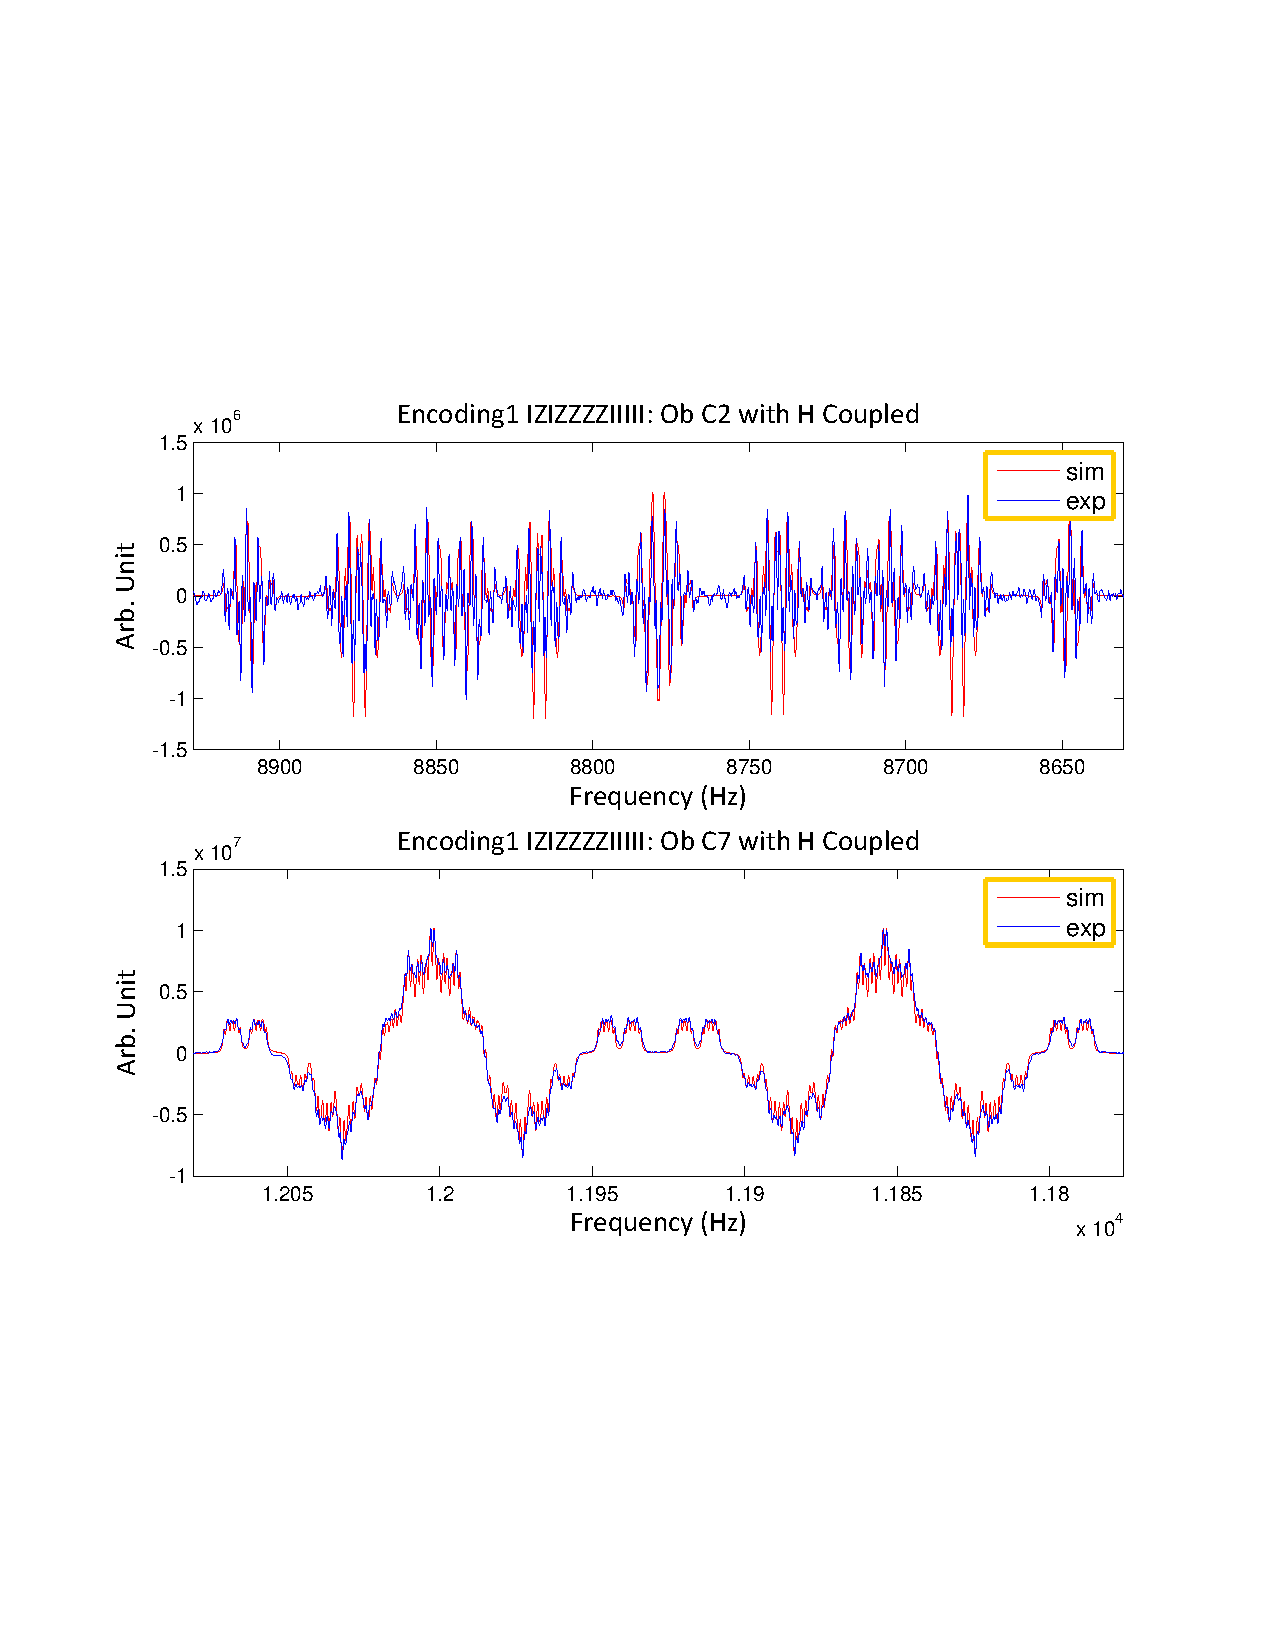
\includegraphics[width=\columnwidth]{Encoding1_C7andC2_SWAP_Hcouple.pdf}
\end{center}
\setlength{\abovecaptionskip}{-0.35cm}
\caption{\footnotesize{Encoding 1 for C2 and C7 without H decoupled. 10 scans.}}\label{2403and2404}
\end{figure}

\clearpage
Exp 2405: Observe C7 after encoding1 and decouple H. NS=1.\\
Exp 2406: Observe C2 after encoding1 and decouple H. NS=1.\\
\textbf{Note compare with undecoupled experiments, for decoupling experiments I just used 1 scan.}

\begin{figure}[htb]
\begin{center}
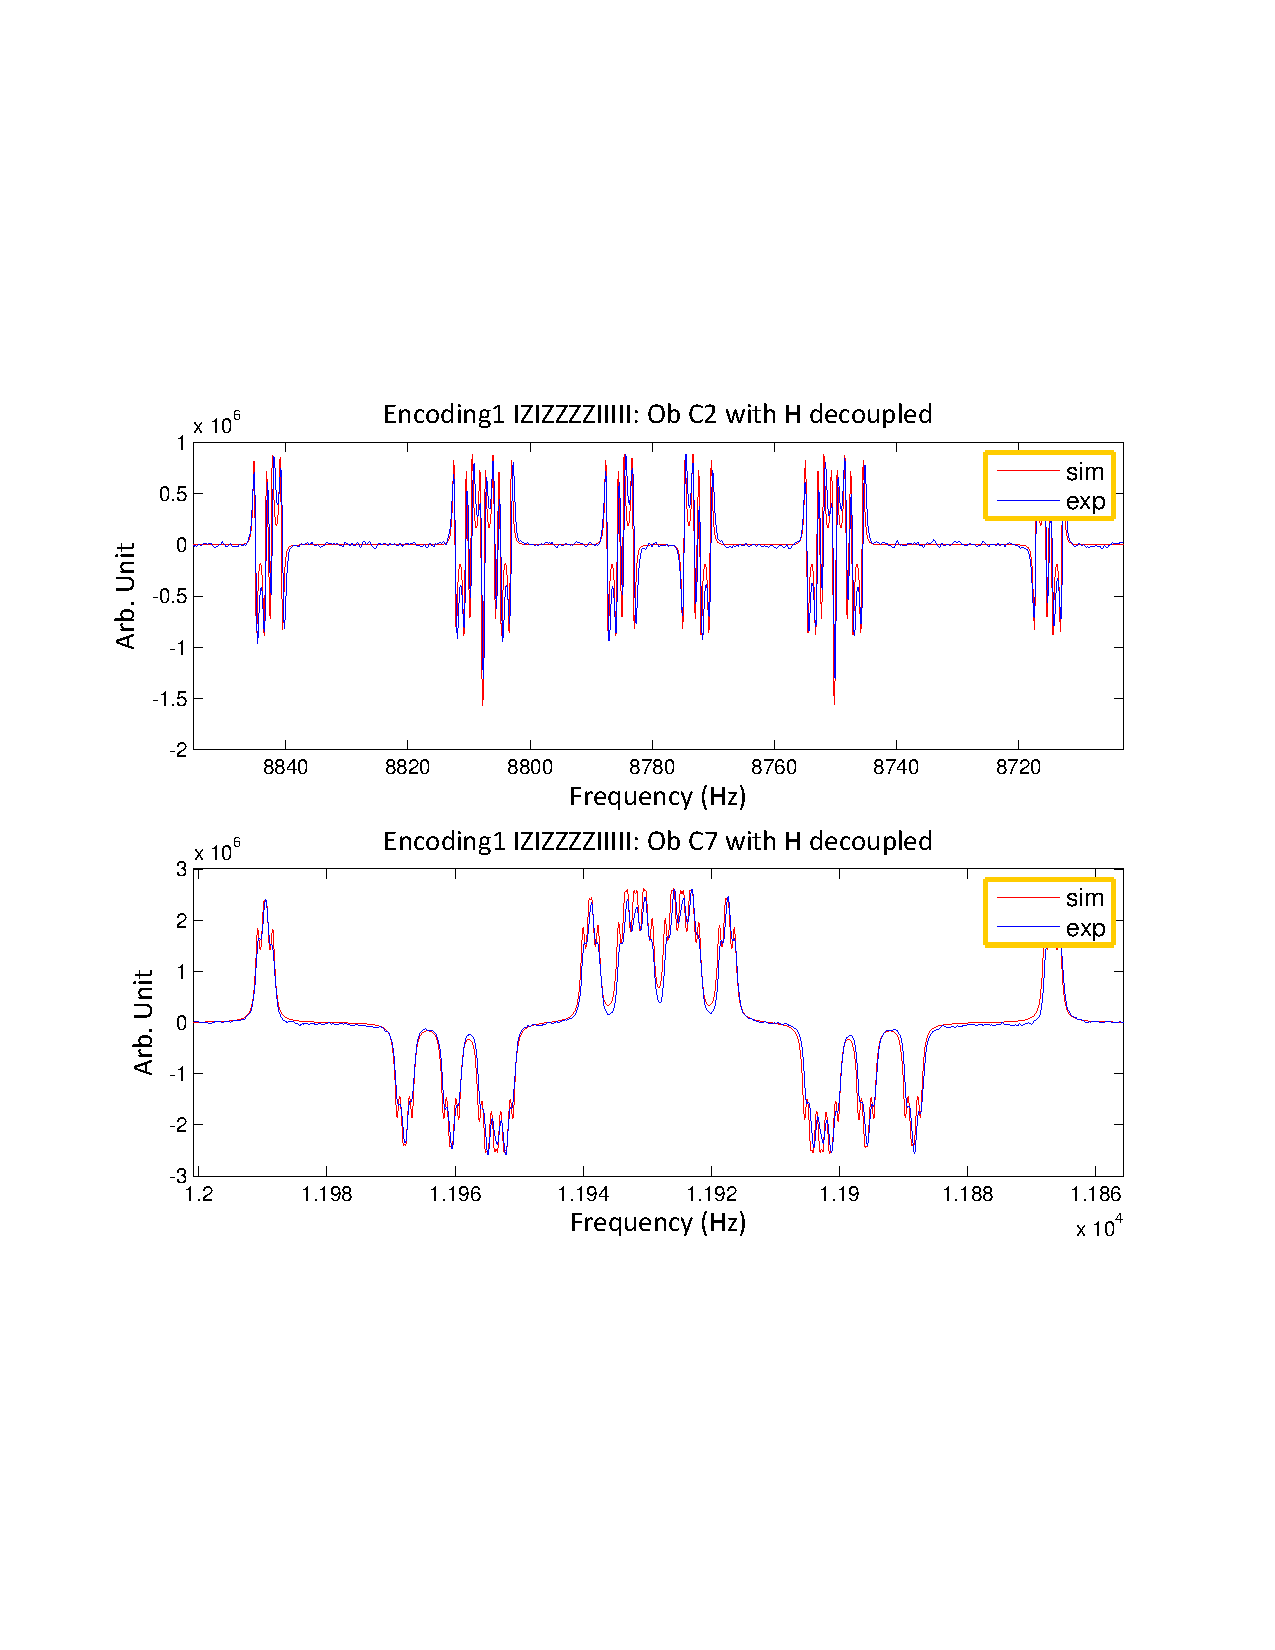
\includegraphics[width=\columnwidth]{Encoding1_C7andC2_SWAP_Hdecouple.pdf}
\end{center}
\setlength{\abovecaptionskip}{-0.35cm}
\caption{\footnotesize{Encoding 1 for C2 and C7 with H decoupled. 1 scan.}}\label{2405and2406}
\end{figure}

\clearpage
Exp 2407: Observe C7 after encoding2. NS=10.\\
Exp 2408: Observe C2 after encoding2. NS=10.\\

\begin{figure}[htb]
\begin{center}
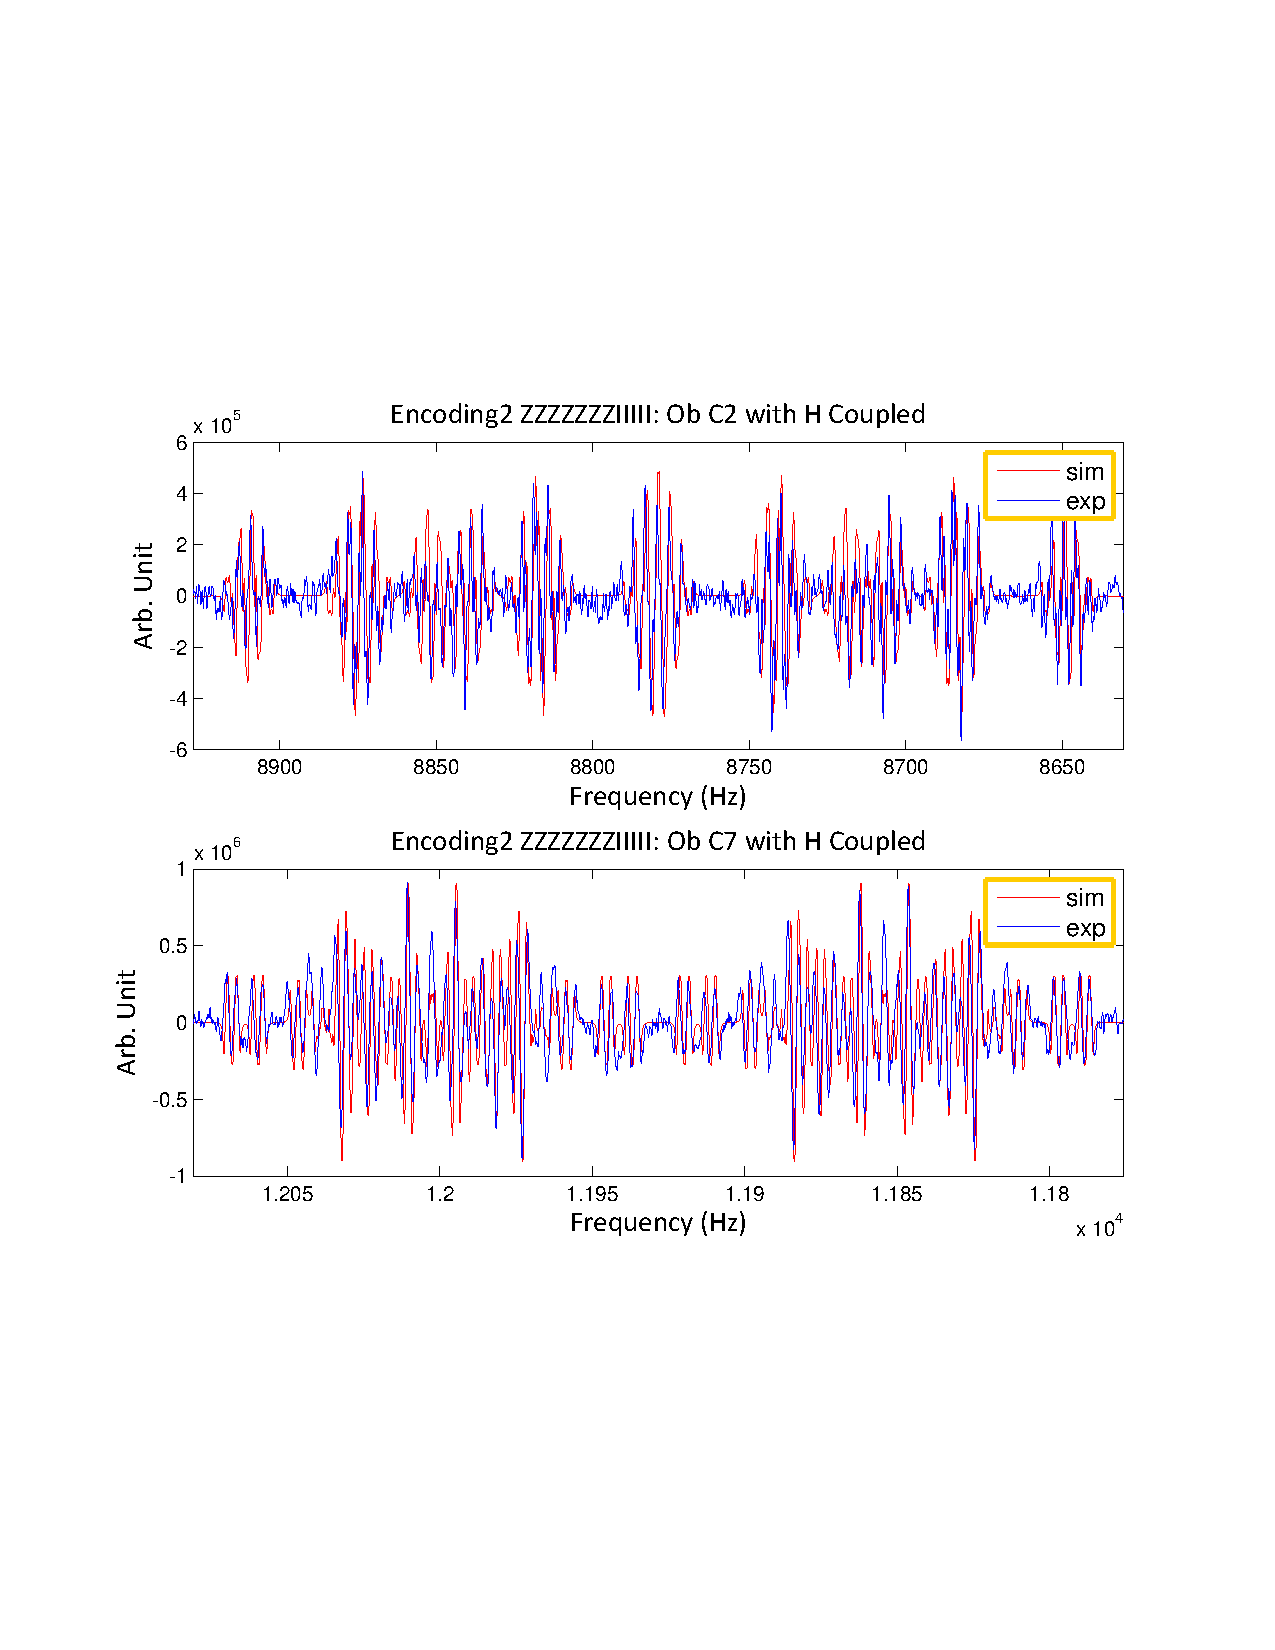
\includegraphics[width=\columnwidth]{Encoding2_C7andC2_SWAP_Hcouple.pdf}
\end{center}
\setlength{\abovecaptionskip}{-0.35cm}
\caption{\footnotesize{Encoding 2 for C2 and C7 without H decoupled. 10 scans.}}\label{2407and2408}
\end{figure}

\clearpage
Exp 2409: Observe C7 after encoding2 and decouple H. NS=1.\\
Exp 2410: Observe C2 after encoding2 and decouple H. NS=1.\\
\textbf{Note compare with undecoupled experiments, for decoupling experiments I just used 1 scan.}

\begin{figure}[htb]
\begin{center}
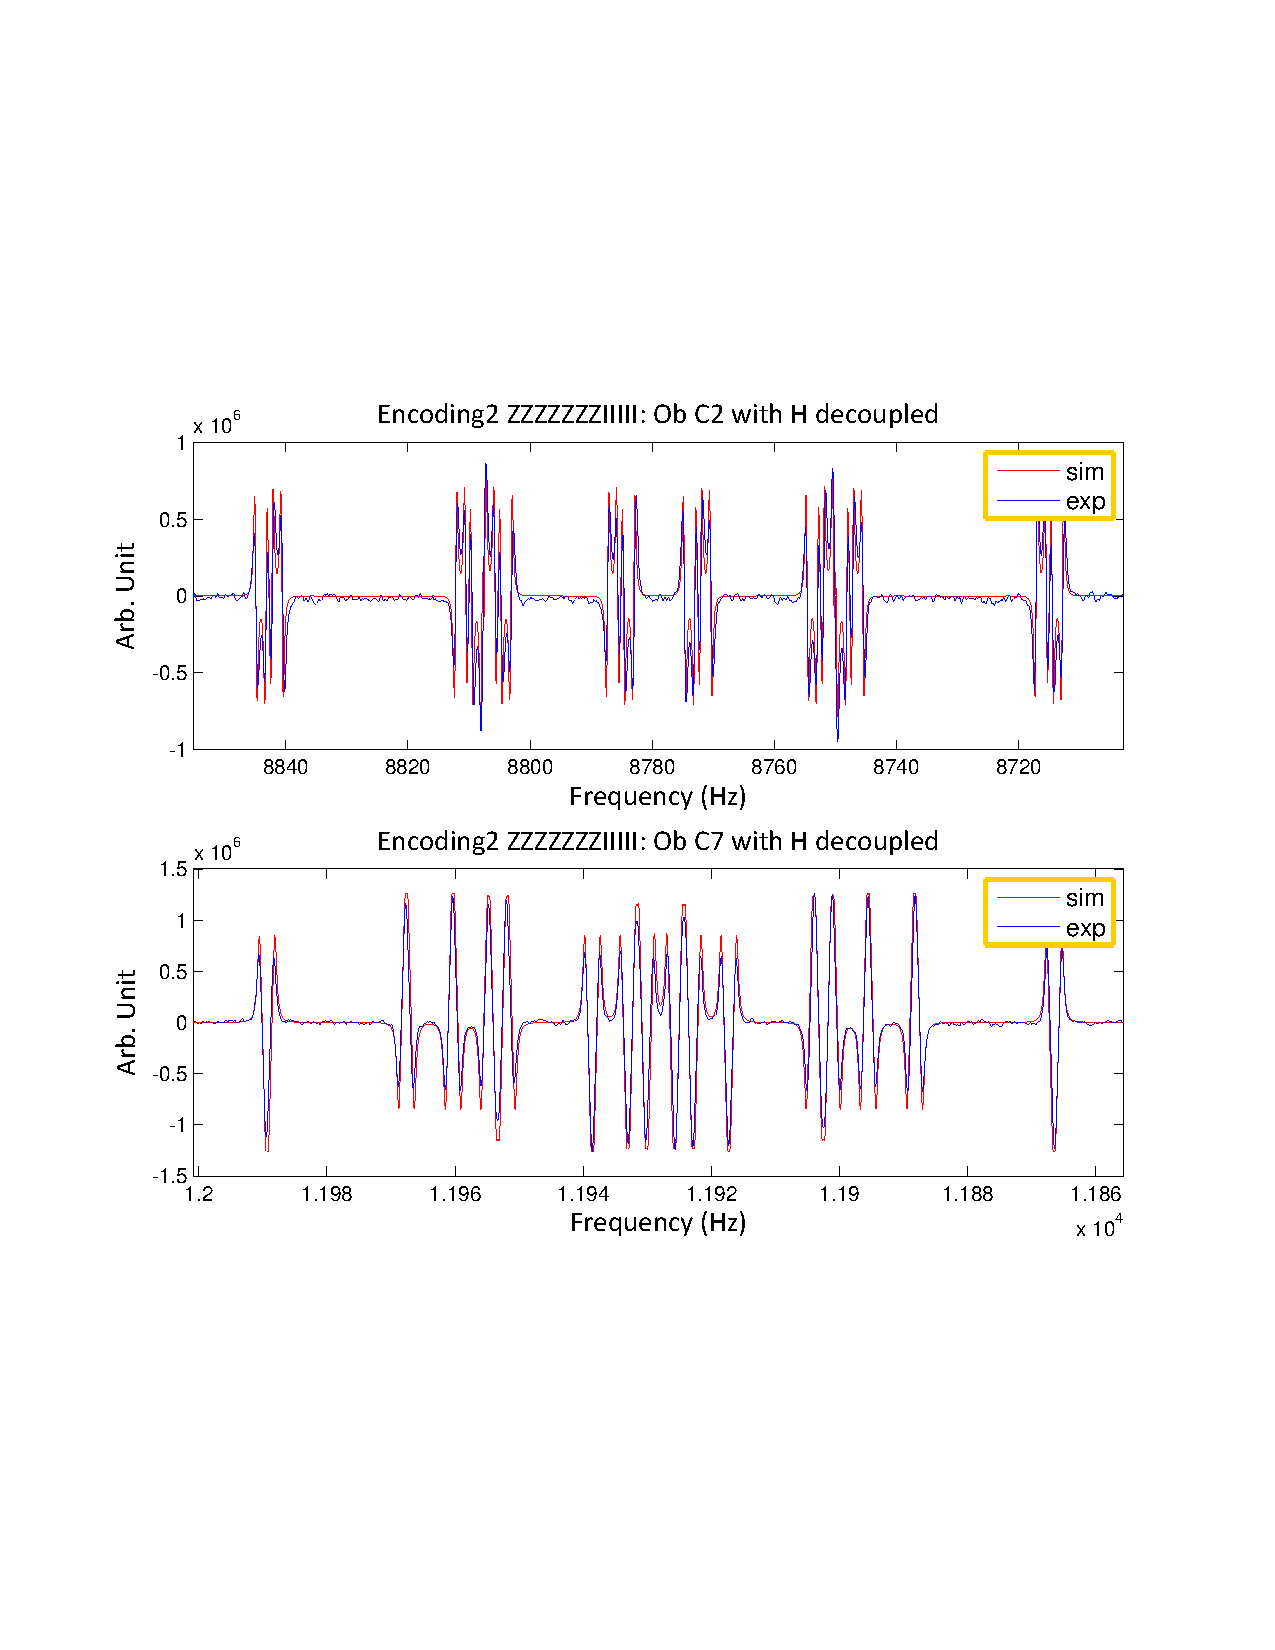
\includegraphics[width=\columnwidth]{Encoding2_C7andC2_SWAP_Hdecouple.pdf}
\end{center}
\setlength{\abovecaptionskip}{-0.35cm}
\caption{\footnotesize{Encoding 2 for C2 and C7 with H decoupled. 1 scan.}}\label{2409and2410}
\end{figure}

\clearpage
Exp 2432: Observe C7 after encoding3 applied twice which generates 7 coherence. NS=10.\\
Exp 2433: Observe C2 after encoding3 applied twice which generates 7 coherence. NS=10.\\

\begin{figure}[htb]
\begin{center}
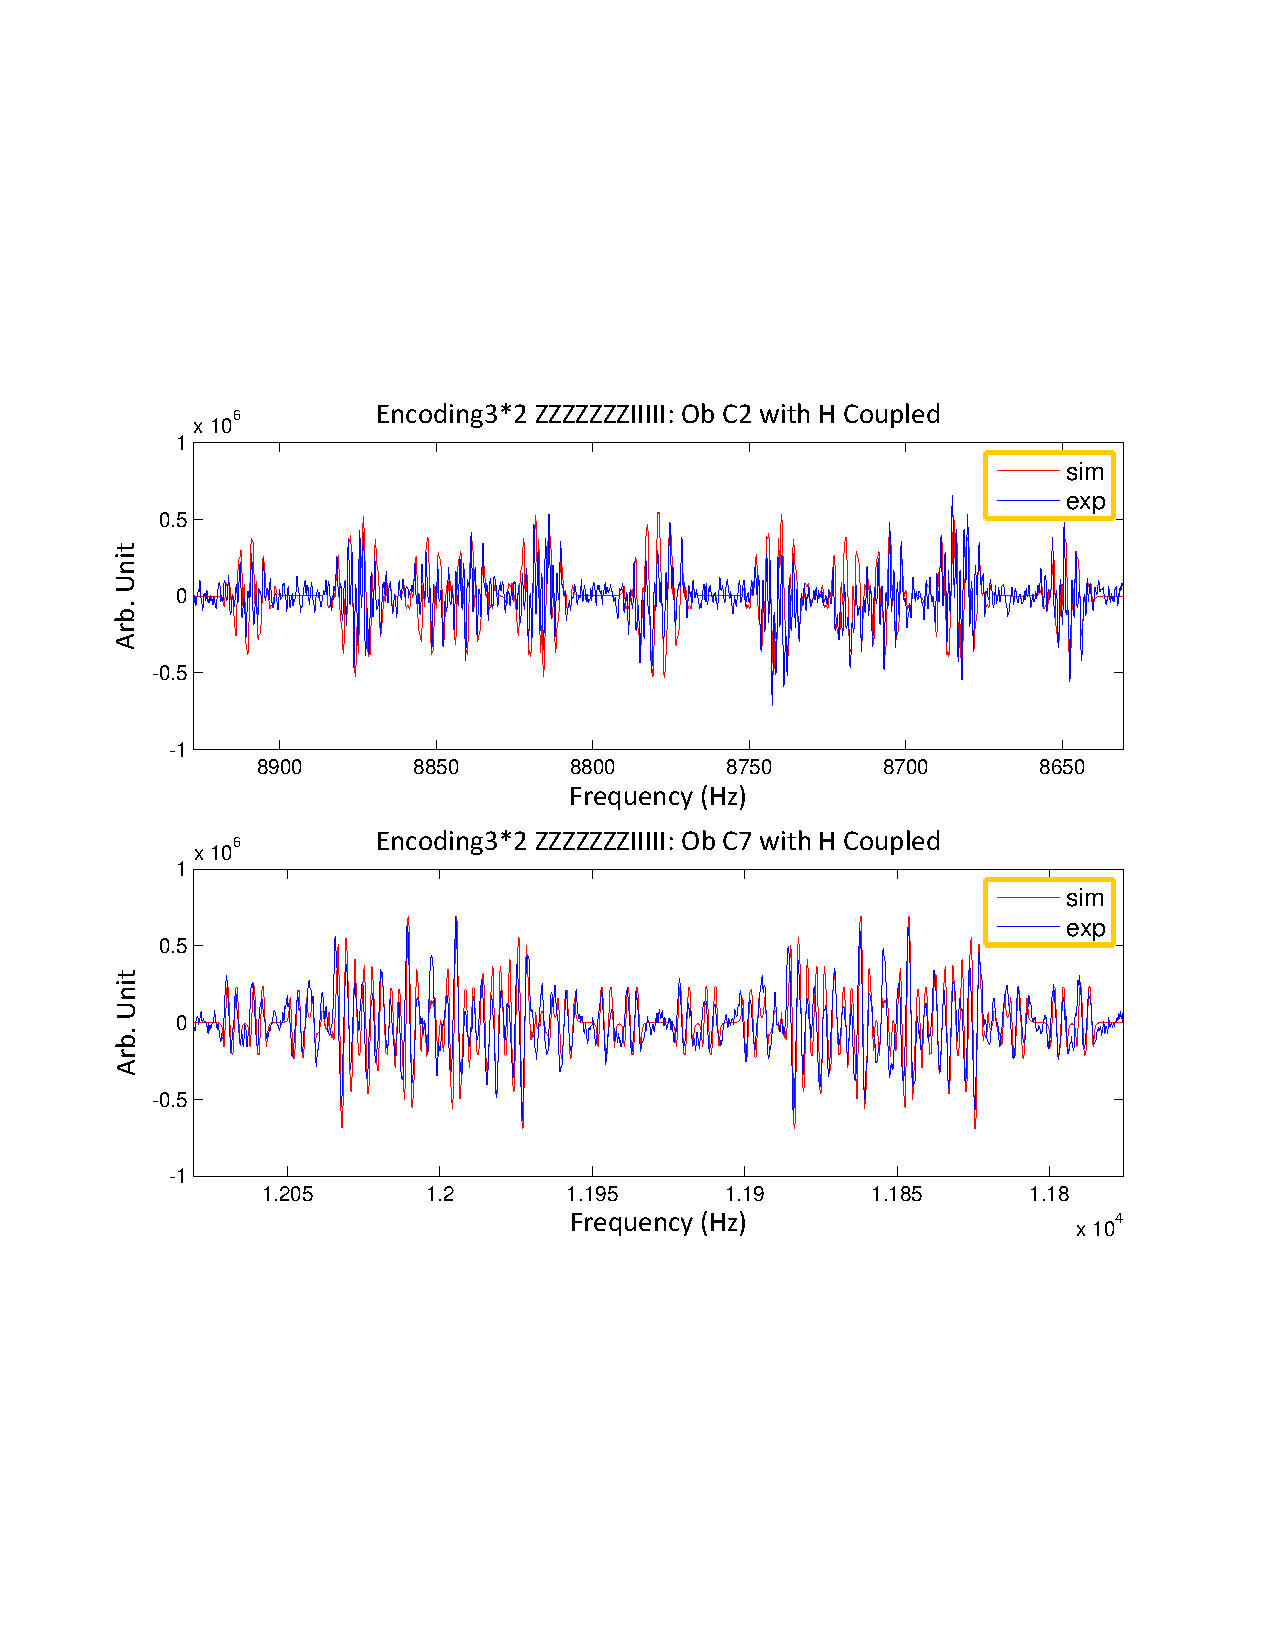
\includegraphics[width=\columnwidth]{Encoding3_Twice_C7andC2_SWAP_Hcouple.pdf}
\end{center}
\setlength{\abovecaptionskip}{-0.35cm}
\caption{\footnotesize{Encoding 3 applied for twice to generate 7 coherence. Observe C2 and C7 without H decoupled. 10 scan.}}\label{2432and2433}
\end{figure}

\clearpage
Exp 2434: Observe C7 after encoding3 applied twice which generates 7 coherence, and decouple H. NS=1.\\
Exp 2435: Observe C2 after encoding3 applied twice which generates 7 coherence, and decouple H. NS=1.\\
\textbf{Note compare with undecoupled experiments, for decoupling experiments I just used 1 scan.}

\begin{figure}[htb]
\begin{center}
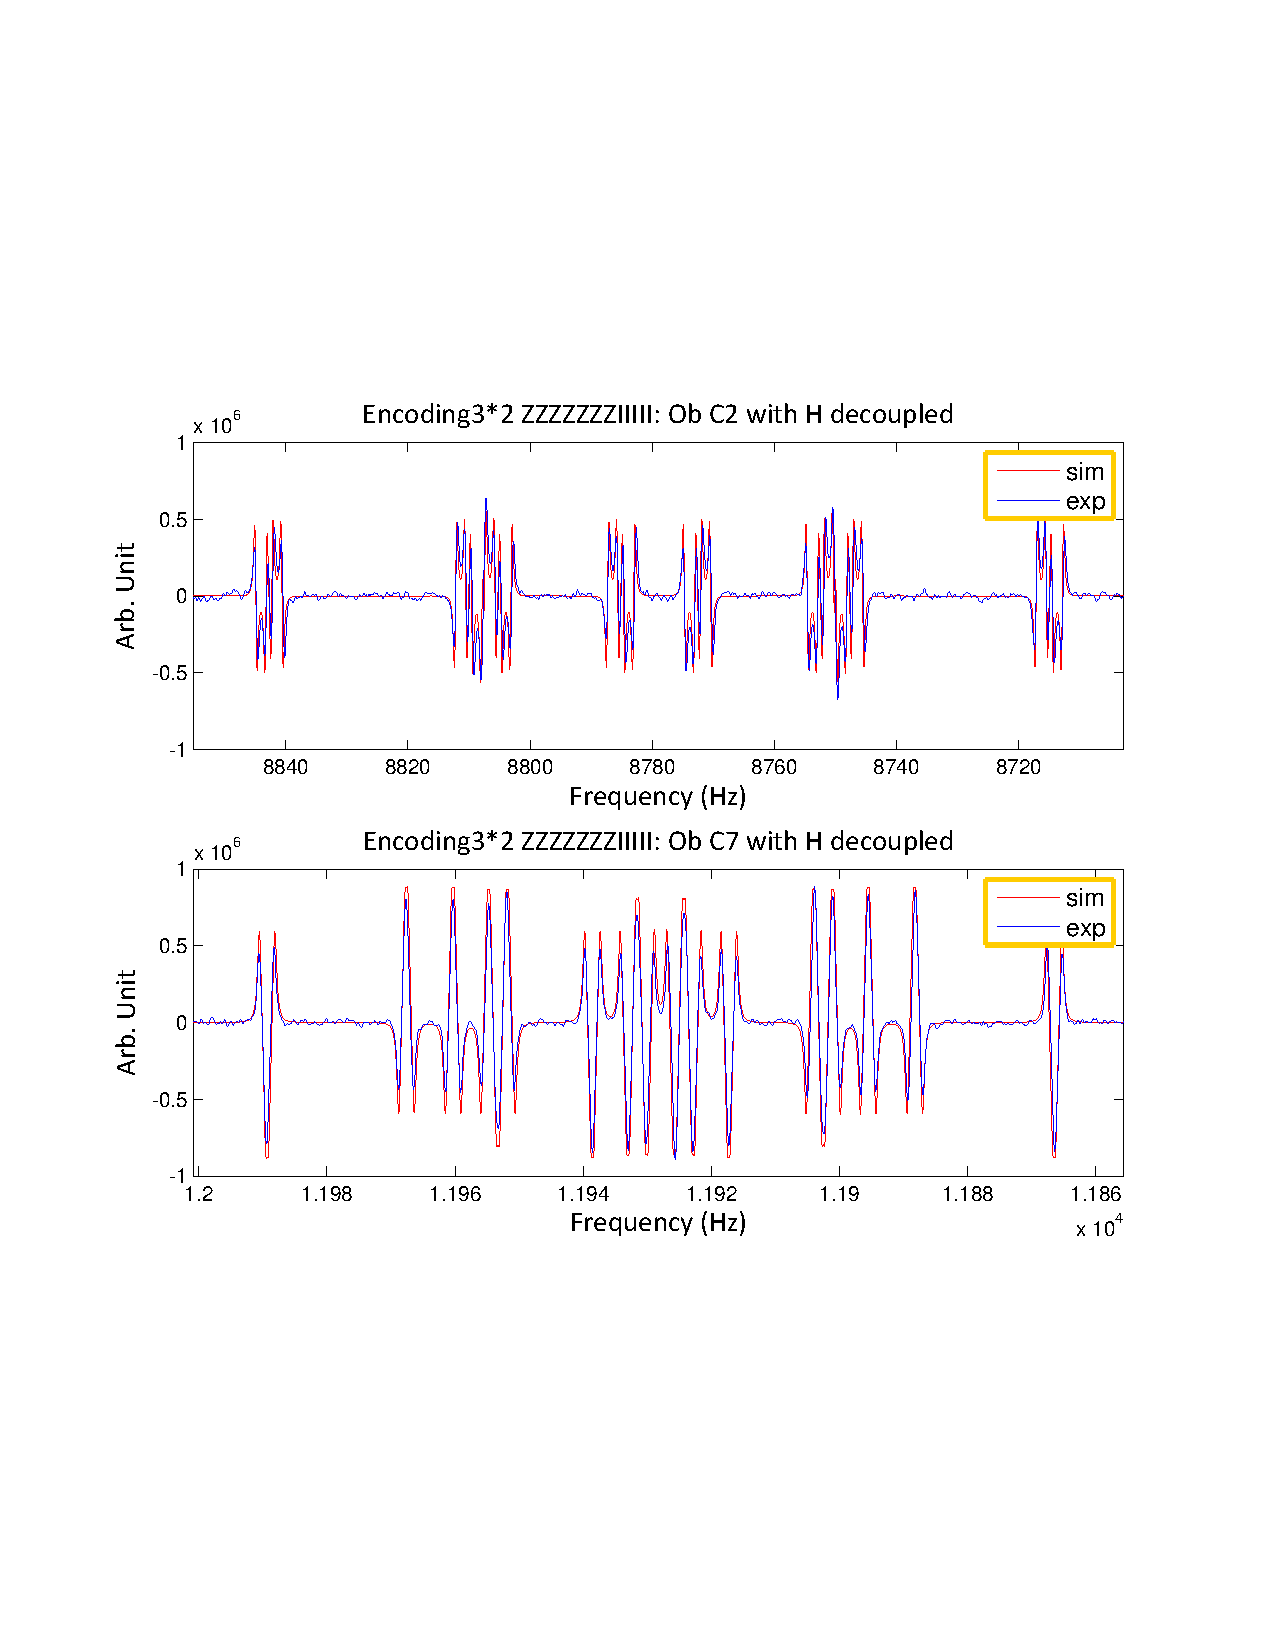
\includegraphics[width=\columnwidth]{Encoding3_Twice_C7andC2_SWAP_Hdecouple.pdf}
\end{center}
\setlength{\abovecaptionskip}{-0.35cm}
\caption{\footnotesize{Encoding 3 applied for twice to generate 7 coherence. Observe C2 and C7 with H decoupled. 10 scan.}}\label{2434and2435}
\end{figure}

\clearpage
Exp 2436: Observe C7 after decoding1new which generates 7 coherence. NS=10.\\
Exp 2437: Observe C2 after decoding1new applied twice which generates 7 coherence. NS=10.\\

\begin{figure}[htb]
\begin{center}
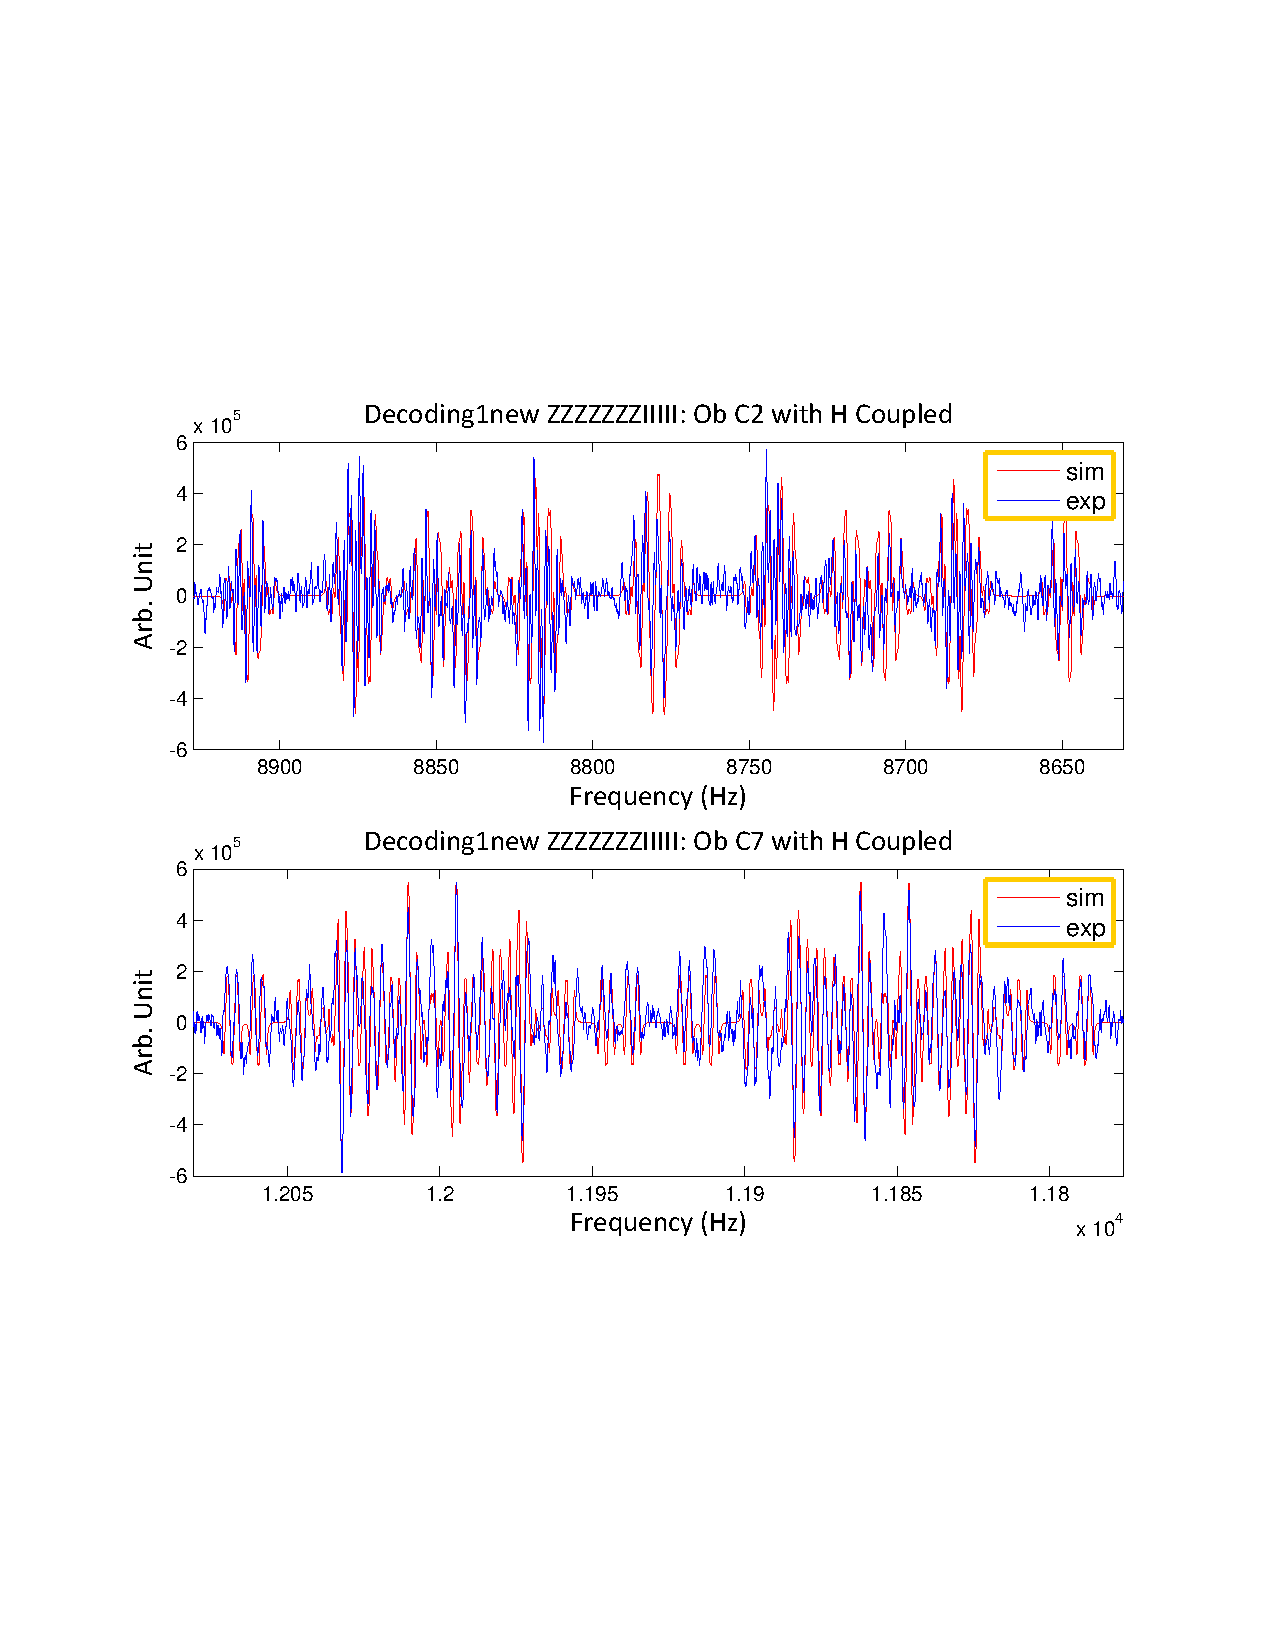
\includegraphics[width=\columnwidth]{Decoding1new_C7andC2_SWAP_Hcouple.pdf}
\end{center}
\setlength{\abovecaptionskip}{-0.35cm}
\caption{\footnotesize{Decoding1new applied to generate 7 coherence. Observe C2 and C7 without H decoupled. 10 scan.}}\label{2436and2437}
\end{figure}

\clearpage
Exp 2438: Observe C7 after decoding1new which generates 7 coherence, and decouple H. NS=1.\\
Exp 2439: Observe C2 after decoding1new which generates 7 coherence, and decouple H. NS=1.\\
\textbf{Note compare with undecoupled experiments, for decoupling experiments I just used 1 scan.}

\begin{figure}[htb]
\begin{center}
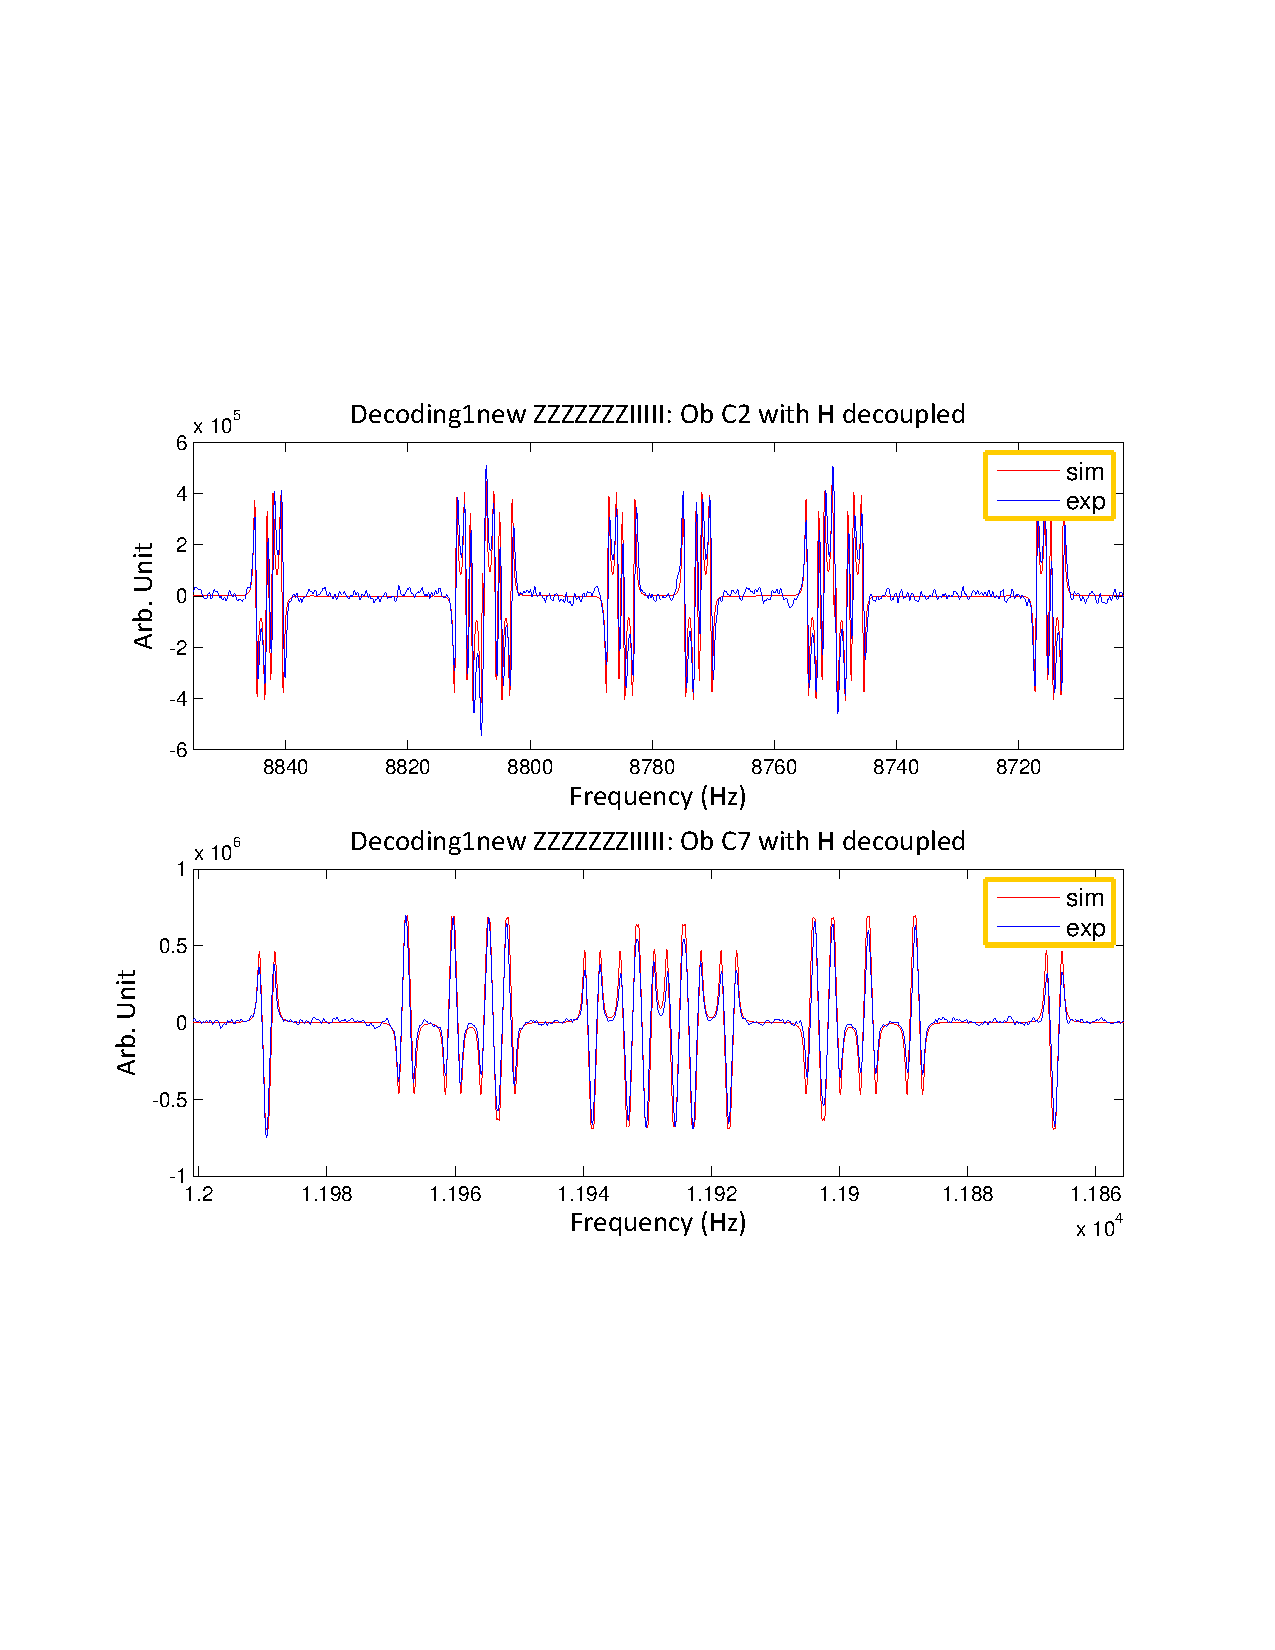
\includegraphics[width=\columnwidth]{Decoding1new_C7andC2_SWAP_Hdecouple.pdf}
\end{center}
\setlength{\abovecaptionskip}{-0.35cm}
\caption{\footnotesize{Decoding1new applied to generate 7 coherence. Observe C2 and C7 with H decoupled. 10 scan.}}\label{2438and2439}
\end{figure}

\clearpage
Exp 2444: Observe C7 after decoding2toend which generates 7 coherence. NS=10.\\
Exp 2445: Observe C2 after decoding2toend which generates 7 coherence. NS=10.\\

\begin{figure}[htb]
\begin{center}
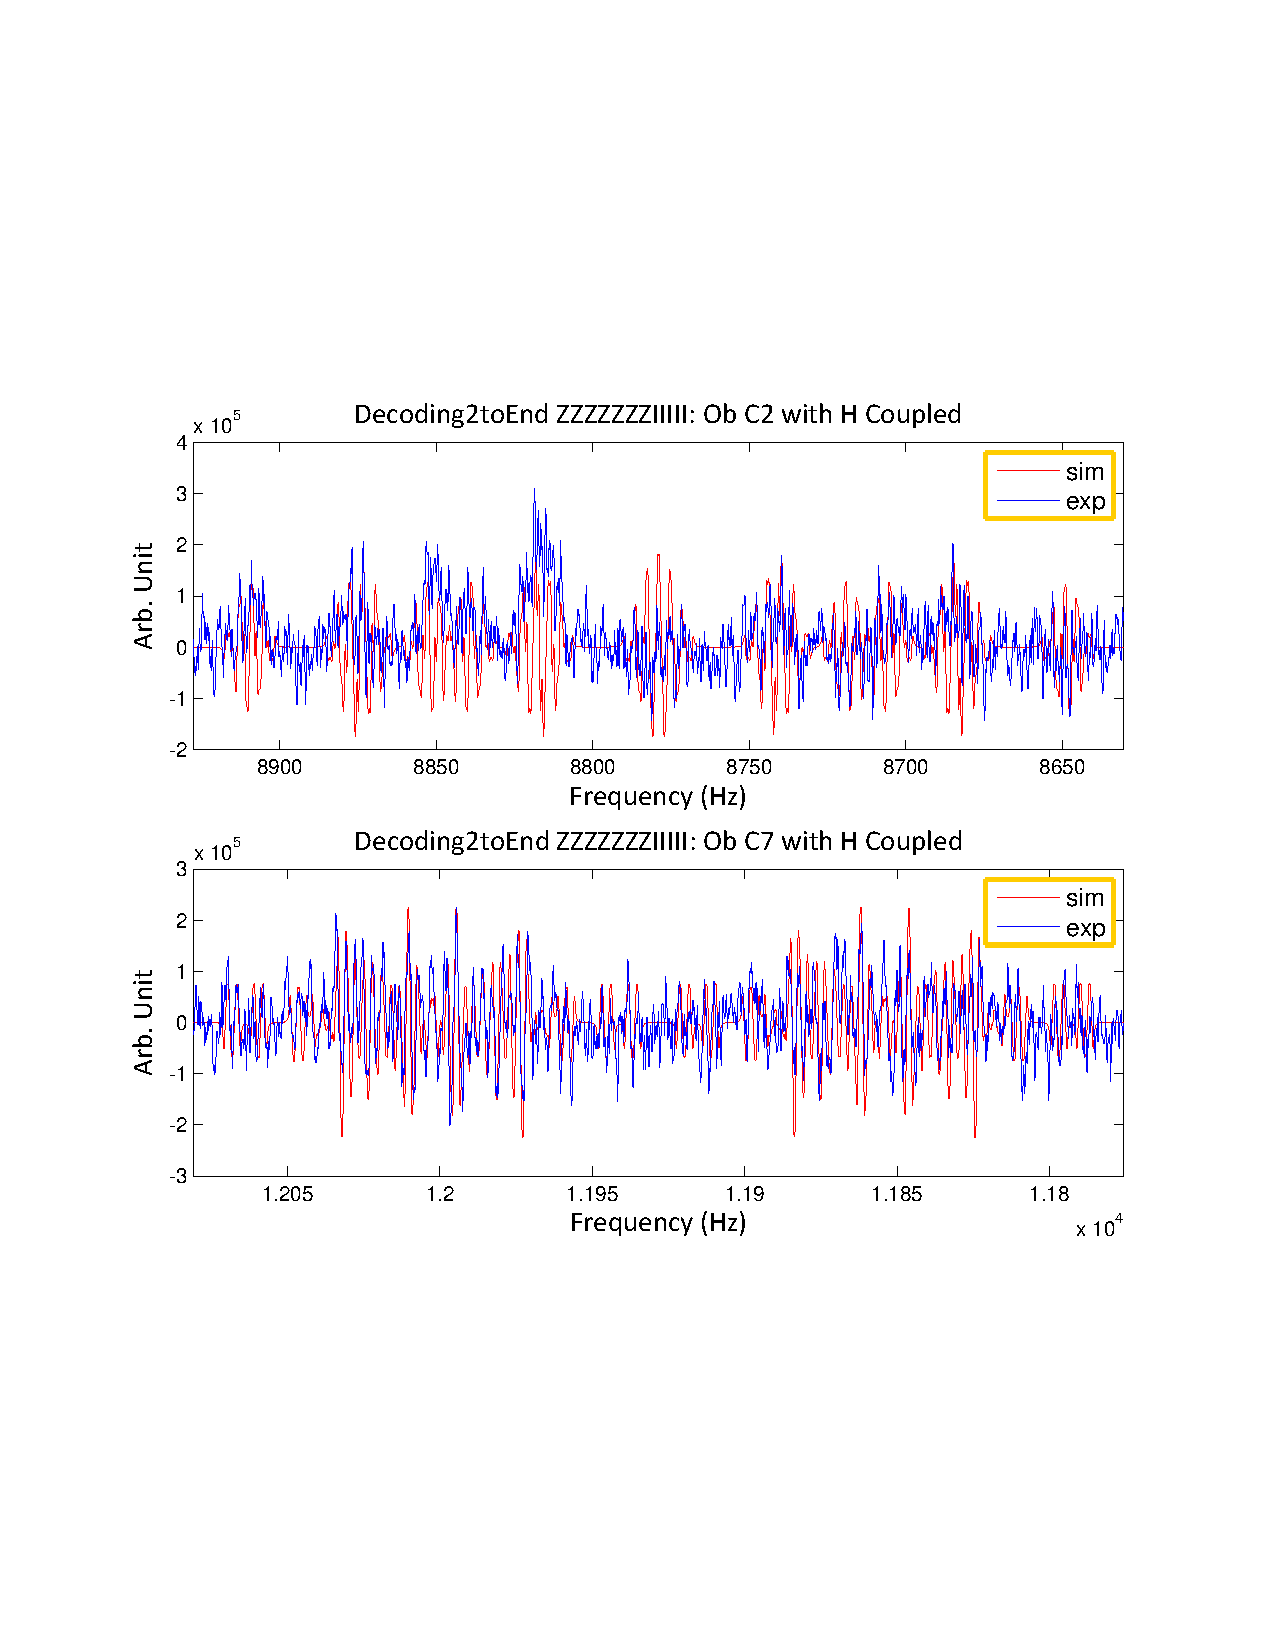
\includegraphics[width=\columnwidth]{Decoding2toEnd_C7andC2_SWAP_Hcouple.pdf}
\end{center}
\setlength{\abovecaptionskip}{-0.35cm}
\caption{\footnotesize{Decoding2toEnd applied to generate 7 coherence. Observe C2 and C7 without H decoupled. 10 scan.}}\label{2444and2445}
\end{figure}

\clearpage
Exp 2446: Observe C7 after decoding2toend which generates 7 coherence, and decouple H. NS=1.\\
Exp 2447: Observe C2 after decoding2toend which generates 7 coherence, and decouple H. NS=1.\\
\textbf{Note compare with undecoupled experiments, for decoupling experiments I just used 1 scan.}

\begin{figure}[htb]
\begin{center}
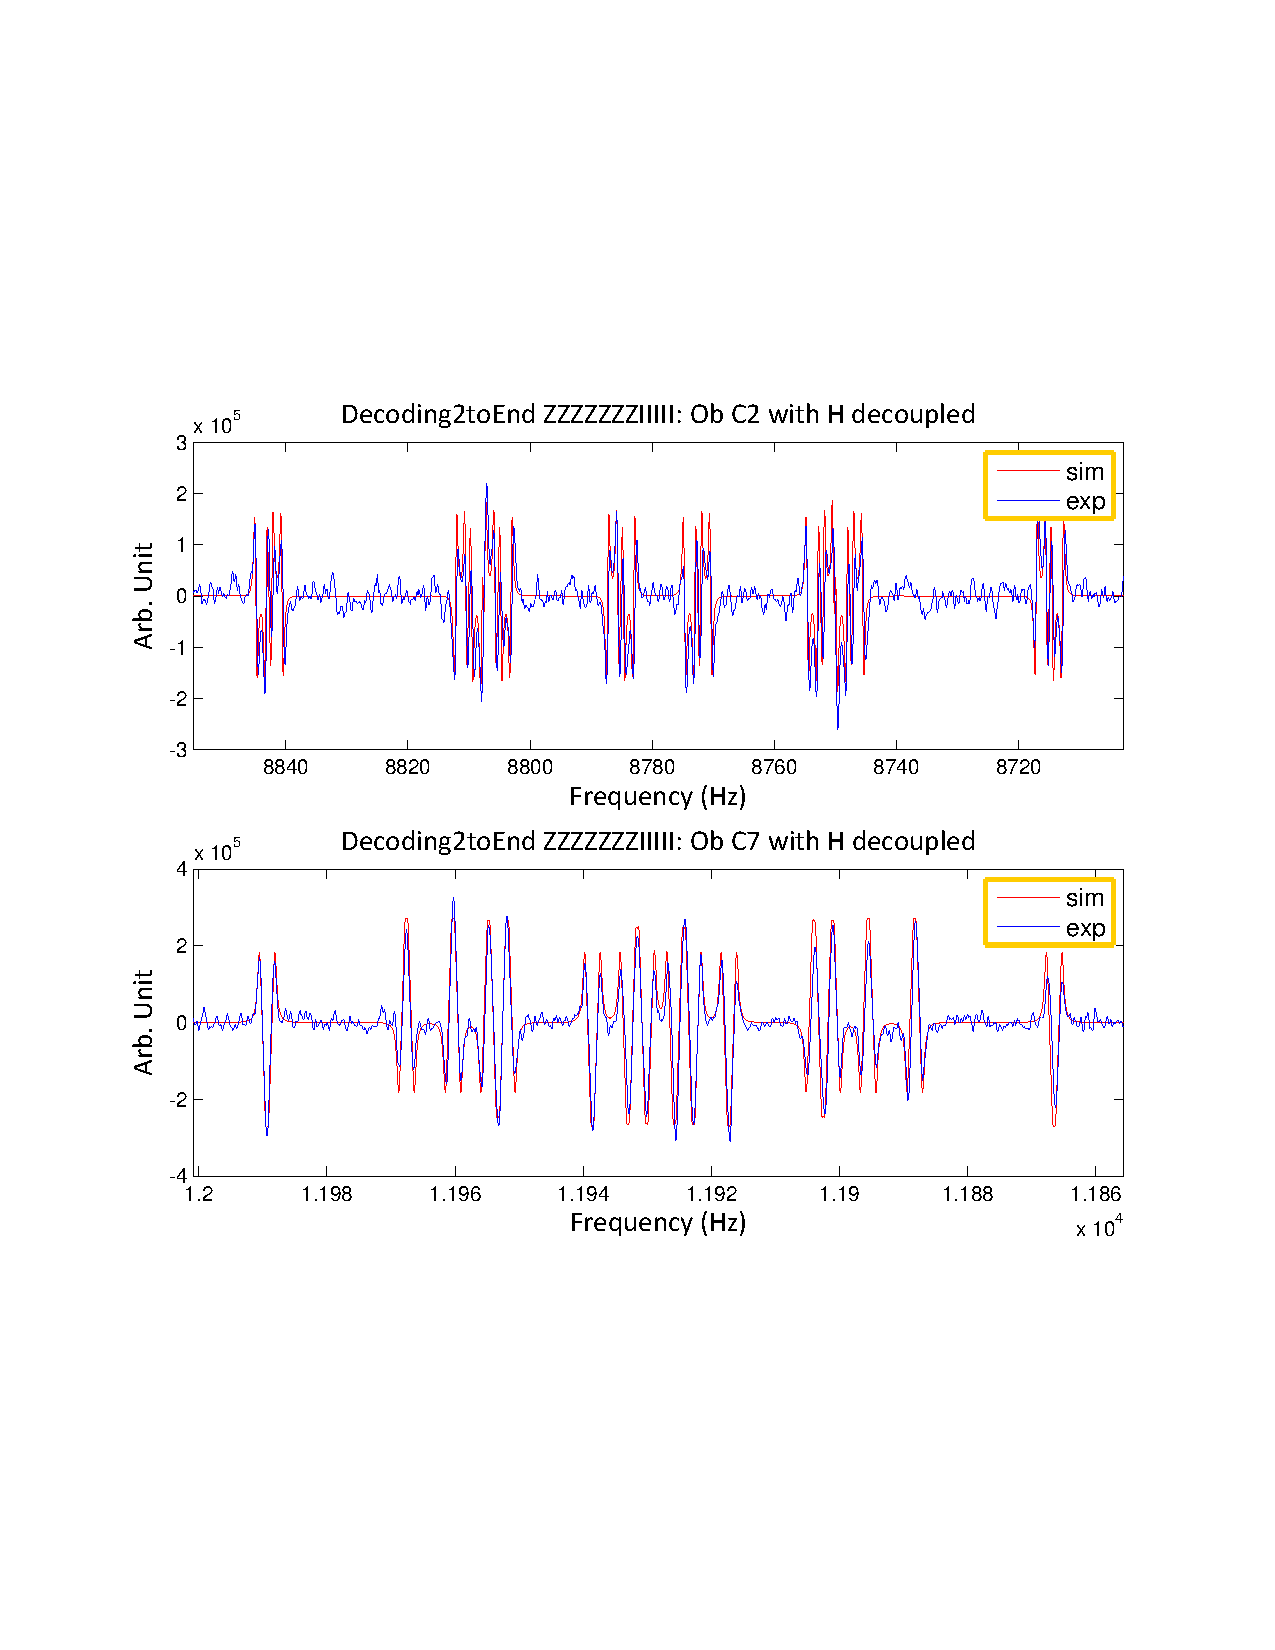
\includegraphics[width=\columnwidth]{Decoding2toEnd_C7andC2_SWAP_Hdecouple.pdf}
\end{center}
\setlength{\abovecaptionskip}{-0.35cm}
\caption{\footnotesize{Decoding2toEnd applied to generate 7 coherence. Observe C2 and C7 with H decoupled. 10 scan.}}\label{2446and2447}
\end{figure}